%% Main presentation %%
% 1. Generate just the presentation (hide notes) and save to slides.pdf
% 2. Generate only the notes (show only nodes) and save to notes.pdf OR? (notes=show/only)
% 3. With Skim, open both slides.pdf and notes.pdf
% 4. Click on slides.pdf to bring it to front.
% 5. In Skim, under "View -> Presentation Option -> Synhcronized Noted Document"
%    select notes.pdf.
% 6. Now as you move around in slides.pdf the notes.pdf file will follow you.
% 7. Arrange windows so that notes.pdf is in full screen mode on your laptop
%    and slides.pdf is in presentation mode on the projector.


%% Title slide content %%
%% Template modfied by Kirsten Wright kirsten.wright@uwaterloo.ca 2024-01-14    %%
%% Based on template by Chris Carmona: carmona@stats.ox.ac.uk ; chriscarmona.me %%

\documentclass[]{beamer} %[notes=show/only]
\usepackage{xcolor, tikz}
\usepackage{geometry}
%\usepackage[outline]{contour}
%\usepackage{adjustwidth}
%\setbeamercovered{transparent=20}
\setbeamertemplate{footline}[frame number]
\setbeamercolor{footline}{fg = blue} 
\setbeamertemplate{navigation symbols}{}
\usetikzlibrary{chains, fit, shadings, shadows, shapes, shapes.geometric, arrows, calc, positioning, shapes.geometric, arrows.meta, patterns, patterns.meta}
% for flow diagram:
\tikzstyle{startstop} = [rectangle, rounded corners, minimum width=3cm, minimum height=1cm,text centered, draw=black, fill=red!30]
\tikzstyle{process} = [rectangle, minimum width=3cm, minimum height=1cm, text centered, draw=black, fill=orange!30]
\tikzstyle{decision} = [rectangle, minimum width=3cm, minimum height=1cm, text centered, draw=black, fill=green!30]
\tikzstyle{arrow} = [thick,->,>=stealth]

\usepackage{adjustbox}

\newcommand\Wider[2][3em]{
% Has 2 parameters, addition to textwidth and content
\makebox[\linewidth][c]{%
  \begin{minipage}{\dimexpr\textwidth+#1\relax}
  \raggedright#2
  \end{minipage}%
  }%
}
% %% Packages %%
% %%%%%%%%%%%%%%%%%%%%%%%%%%%%%%%%
% %%%%%%%%%%%%%%%%%%%%%%%%%%%%%%%%

% \usepackage{tikz}
% \usepackage[UKenglish]{babel}
% \usepackage[utf8]{inputenc} % so we can input characters with accents (e.g. ő)

% \usepackage{statsbeamer}

% \usepackage{graphicx} % ease graphics management
% % \graphicspath{{images/}} % define folder with images
% % \graphicspath{{fig/}} % define folder with images
% \usefonttheme{serif} % change font to allow \textbf{}
% \usepackage{charter} % Nicer fonts

% \usepackage{amsmath,amsthm,amssymb} % for math equations

% % \usepackage{natbib} % richer citation
% \usepackage{breakcites} % avoid overfull hbox for long cites


%% Information (author, title, etc.) %%
% \setbeamerfont{title}{size*={2pt}}
\title{ Financialization of the Housing Market: A Contribution to Modern Urban Rent Theory}
% \author{Kirsten Wright} %\underline{Alyssa P. Hacker} \inst{1} \and Ben Bitdiddle \inst{2} \and Lem E. Tweakit \inst{2}}
\author{
  Author: Kirsten Wright \\
  Supervisors: Jangho Yang, Sean Geobey
}
% \institute{PhD Thesis Defensae}
% \institute{PhD Thesis Defense \\[1ex] University of Waterloo}
\institute{SYDE Graduate Seminar \\[1ex] University of Waterloo}
%\date{February 10, 2024}
\date{May 22, 2024}
% \title[Short Title]{% short title for footer
%     Long and Descriptive Title
%     \vspace{0.5cm}
% }
% \author{ Your Name \and Your Collaborator}
% \institute{
%         \textit{Department of Statistics}\\
%         \textit{University of Waterloo}
%         \vspace{0.5cm}
% }
% \date[Venue and Date]{% short date for footer
%     Venue, Date
% }
\begin{document}{
    %\setbeamertemplate{footline}{framenumber}
    \setbeamertemplate{headline}{}
    \setbeamercolor{background canvas}{bg=white}
    \maketitle   
}

%%%%%%%%%%%%%%%%%%%%%%%%%%%%%%%%%%%%%%%%%
% \begin{frame}{Financialization}
%     \centering
%     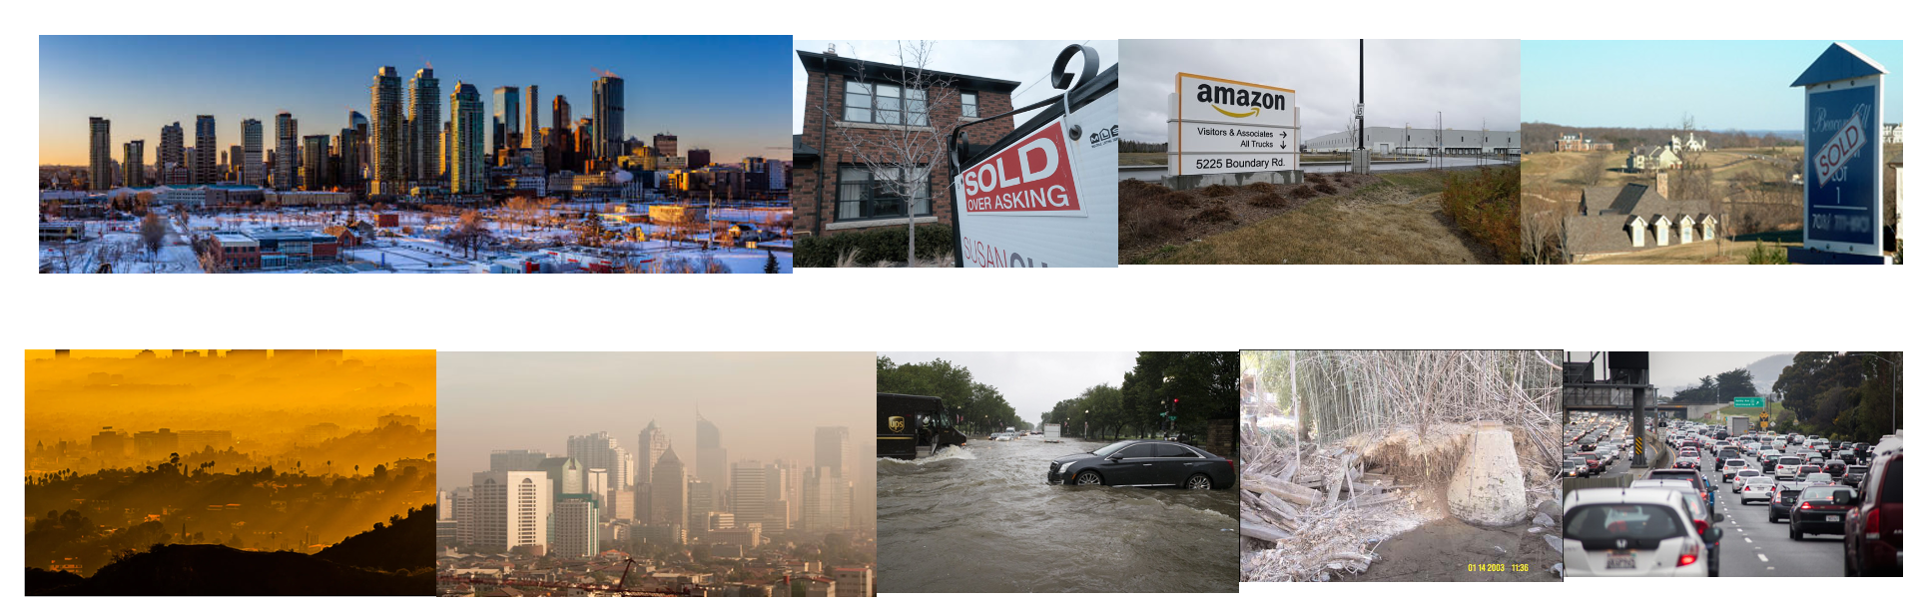
\includegraphics[scale=0.167]{fig/example_figures/pictures-ex-1.png}
%     \vspace{-2.5em} % Adjust the vertical space as needed
%     \begin{flushright}
%         \tiny{Source: Dawn Parker}
%     \end{flushright}
% \end{frame}

%%%%%%%%%%%%%%%%%%%%%%%%%%%%%%%%%%%%%%%%%
\begin{frame}{Financialization: 
the capture of flows of surplus by financial actors.}
\begin{itemize} \Large 
    \item Surplus is produced by bringing people together in the city 
    \item Claiming surplus works by capturing land rents % is at the heart of what’s happening in urban centers.  
    \item Financialization is achieved through the creation of financial instruments, like REITs, and mortgages 
\end{itemize}

\end{frame}

%%%%%%%%%%%%%%%%%%%%%%%%%%%%%%%%%%%%%%%%%
\begin{frame}
\begin{figure}[!ht]
\centering
\resizebox{0.85\textwidth}{!}{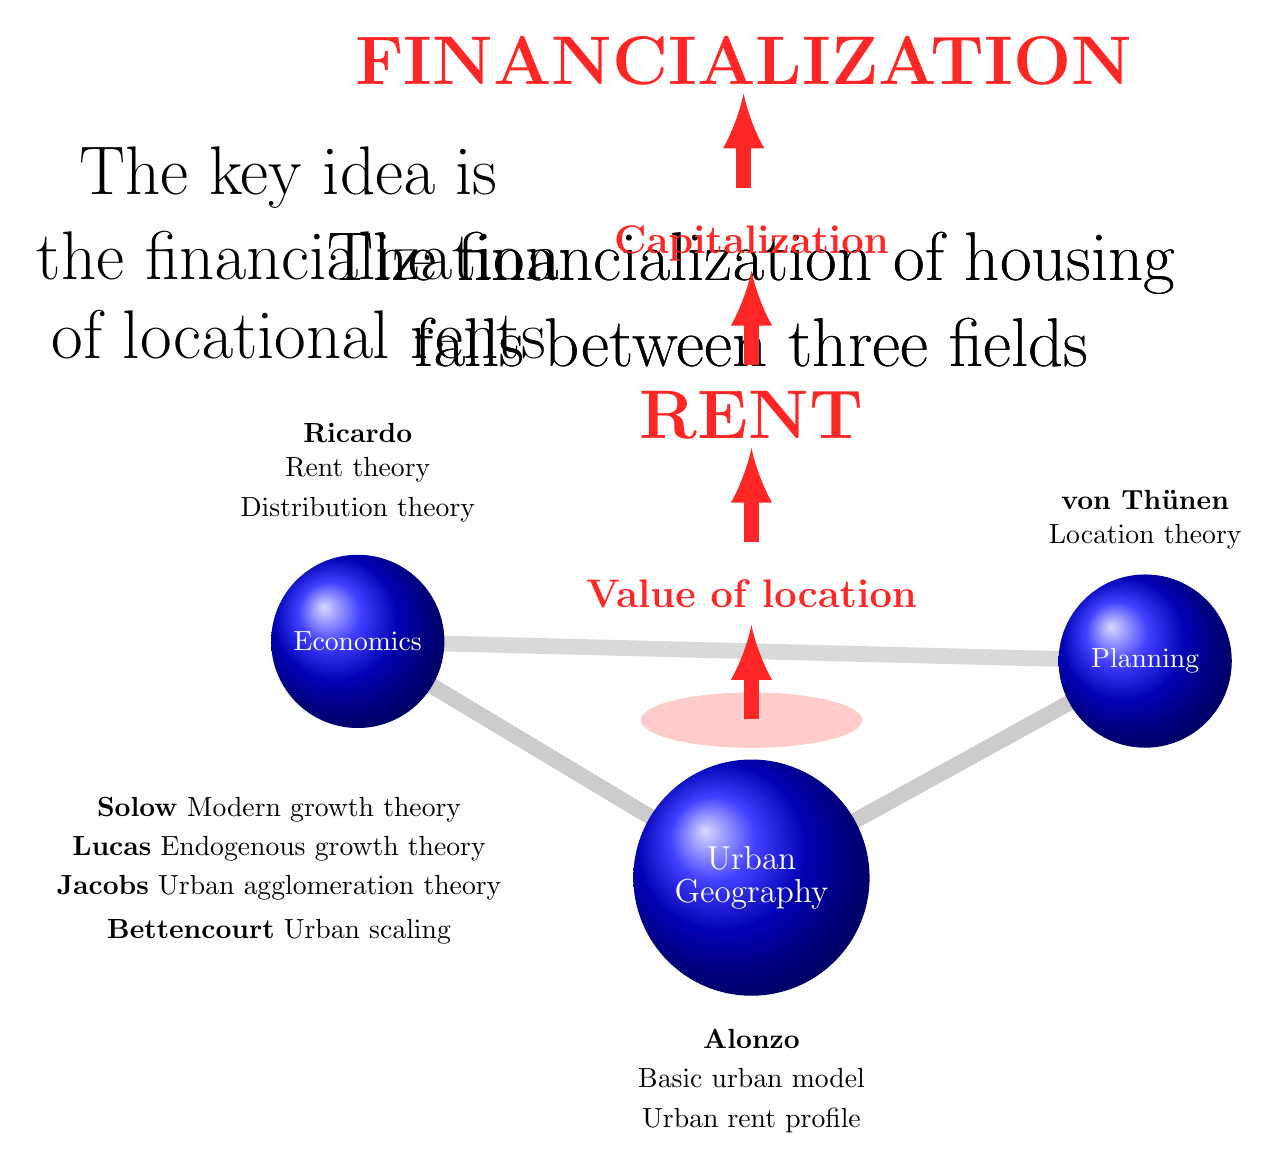
\begin{tikzpicture}{scale=.5}
% Find color for ball. Stop line short of node
\coordinate (planning) at (5,.75); % Preface
\coordinate (economics) at (-5,1); 
\coordinate (Ricardo) at (-5,1.4);
\coordinate (Solow) at (-6,1.25);
\coordinate (geography) at (0,-2); % History
\coordinate (finance) at (0,5); 

\draw [line width=2mm, black!15, ] (planning)--(economics);
\draw [line width=2mm, black!20, ] (geography)--(economics);
\draw [line width=2mm, black!20, ] (geography)--(planning);
%\draw [line width=2mm, black!25, ] (geography)--(finance);
%\draw [line width=2mm, black!20, ] (planning)--(finance);
%\draw [line width=2mm, black!20, ] (finance)--(economics);
%color=black!60!red
%\shade [ball color=blue!70] (5,5) circle (1.1cm)node[white] {\textbf{Planning}};
 
\node [circle,shading=ball,  minimum width=2.2cm, white, align=center] (ball) at (planning) {Planning};
\node [circle, shading=ball, minimum width=2.2cm, white, align=center] (ball) at (economics) {Economics};
\node [circle,shading=ball, minimum width=3cm, white, align=center] (ball) at (geography)[text width=2cm] {\large Urban \\ Geography};
%\node [circle, shading=ball, minimum width=2.4cm, white, align=center] (ball) at (finance)[text width=2cm] {Finance};
%\node at (-.3,-.1) [red] {\Large \textbf{RENT}};

\fill[red!20] (0,0) ellipse (40pt and 10pt);

\onslide<1>
{\node at (0, 5.8)[align=center, font=\Huge ]{The financialization of housing};
\node at (0, 4.8)[align=center, font=\Huge]  {falls between three fields};
};

\onslide<2>
{\node at (0, 5.8)[align=center, font=\Huge ]{The financialization of housing};
\node at (0, 4.8)[align=center, font=\Huge]  {falls between three fields};
};
% \onslide<2>{\node at (0, 5.8)[align=center]{\Huge I draw on  theories };
% \node at (0, 4.8)[align=center]{\Huge from multiple fields};
% };

\onslide<3>
{\node at (-5.75, 6.9)[align=center]{\Huge The key idea is };
\node at (-5.75, 5.9)[align=center]{\Huge the financialization};
\node at (-5.75, 4.9)[align=center]{\Huge  of locational rents};
};

\pause


\node at (planning) [above=1.8cm] {\textbf{von Th\"unen}};
\node at (planning) [above=1.3cm] {Location theory};

\node at (Ricardo) [above=2cm,]   {\textbf{Ricardo}};
\node at (Ricardo) [above=1.5cm] {Rent theory};
\node at (Ricardo) [above=1.0cm] {Distribution theory};

% \node at (Solow) [below=1.6cm, align=left] {\textbf{Solow:}};
\node at (Solow) [below=2.1cm, align=left] {\textbf{Solow} Modern growth theory};
\node at (Solow) [below=2.6cm, align=left] {\textbf{Lucas} Endogenous growth theory};
\node at (Solow) [below=3.1cm, align=left] {\textbf{Jacobs} Urban agglomeration theory};
\node at (Solow) [below=3.65cm, align=left] {\textbf{Bettencourt} Urban scaling};

\node at (geography) [below=1.8cm] {\textbf{Alonzo}};
\node at (geography) [below=2.3cm] {Basic urban model};
\node at (geography) [below=2.8cm] {Urban rent profile};
%\node [circle, shading=ball, minimum width=2.4cm, white, align=center] (ball) at (finance)[text width=2cm] {Finance};


\pause

%\node[red]at (1.2,0) {\large SPACE};
\begin{scope}[shift={(0,-.34)}]
\draw [line width=2mm, red!85, -latex ] (-.1, 7.1)--++(0,1.2)node[above=-.1] {\Huge \textbf{FINANCIALIZATION}};
\draw [line width=2mm, red!85, -latex ] (0, 4.85)--++(0,1.2)node[above=-.1] {\Large \textbf{Capitalization}};
\draw [line width=2mm, red!85, -latex ] (0, 2.6)--++(0,1.2)node[above=-.1] {\Huge \textbf{RENT}};
\draw [line width=2mm, red!85, -latex ] (0, .35)--++(0,1.2)node[above] {\Large \textbf{Value of location}};
%\draw [line width=2mm, red!85, -latex ] (0, -2)--++(0,-.8)node[above=-.1]  {\Large \textbf{SPACE}};
\end{scope}
\end{tikzpicture}


% % JUST THE BOTTOM 3 BALLS FOR PLANNING, ECONOMICS AND URBAN GEOGRAPHY
% \begin{figure}
% \begin{tikzpicture}{scale=.5}
% % find color cotrol for ball. Tind way to stop line short of node
% \coordinate (planning) at (-5,1);%PREFACE
% \coordinate (economics) at (5,.75);%
%  \coordinate (geography) at (-.5,-2); %history
% \coordinate (finance) at (0,5); %

% \draw [line width=2mm, black!15, ] (planning)--(economics);
% \draw [line width=2mm, black!20, ] (geography)--(economics);
% \draw [line width=2mm, black!20, ] (geography)--(planning);

% %\draw [line width=2mm, black!25, ] (geography)--(finance);
% %\draw [line width=2mm, black!20, ] (planning)--(finance);
% %\draw [line width=2mm, black!20, ] (finance)--(economics);
% \node [circle,shading=ball, minimum width=2.1   cm, white, align=center] (ball) at (planning) {Planning};
% \node [circle,shading=ball, minimum width=2.2cm, white, align=center] (ball) at (economics) {Economics};
% \node [circle,shading=ball, minimum width=3cm, white, align=center] (ball) at (geography)[text width=2cm] {\large Urban\\ Geography};
% %\node [circle, shading=ball, minimum width=2.4cm, white, align=center] (ball) at (finance)[text width=2cm] {Finance};

% \node at (-.3,-.1) [red] {\Large \textbf{Space}};
% \end{tikzpicture}
% \caption{The common concern of three fields topic }
%     \label{fig-three-fields}
% \end{figure}}
\label{fig:fieldsplus}
\end{figure}
\end{frame}

%%%%%%%%%%%%%%%%%%%%%%%%%%%%%%%%%%%%%%%%%
\begin{frame}{Ricardian rent theory}
\begin{itemize}\Large
    \item Ricardo examined production and distribution in an agricultural society
    \item \textbf{Farmers} pay to transport \textbf{product} to the \textbf{market}
    \item All surplus went to the class of landowners as rent
\end{itemize}
\begin{centering}  \vspace{0cm}\hspace{1cm} 
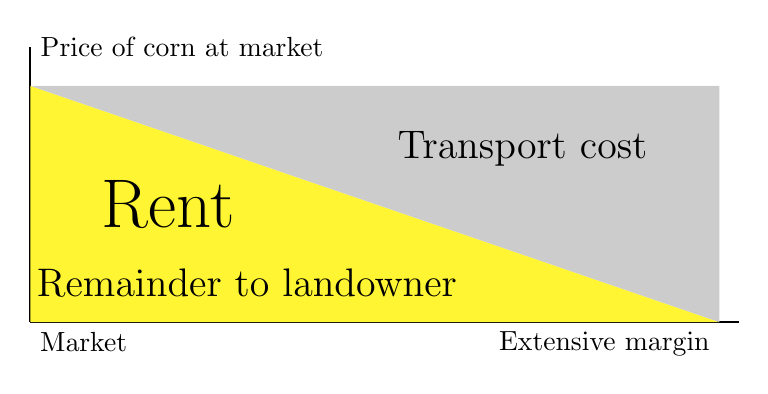
\begin{tikzpicture}[domain=0:2]
\node at (.25,0) [below right, text width=4cm, black ]{Market};
% \node at (.25,-1.) [below right, text width=4cm, black ]{center };
% \node at (.25,-2) [below right, text width=4cm, black ]{\Huge Market};
\draw[thick ] (9.25,0)  -- (.25,0);

\draw[thick ] (.25,0)  -- (.25, 3.5)node[ right ]{Price of corn at market};
\fill[yellow!80]  (.25,0) --(.25,3)--(9,0)node[below left, black]{ Extensive margin} --cycle;
\fill[gray!40] (9,3) --(.25,3)--(9,0) --cycle;

\node  at (2.,1.5)[font=\Huge ]{Rent};
\node  at (3,.5)[font=\Large]{ Remainder to landowner};
\node  at (6.5,2.2){\Large Transport cost};
% \draw[latex-, line width=1.5mm] (9,-.25) --(9, -2);
% \draw[-latex, line width=.75mm] (.25,-4)node[above]{distance from centre} --(6,-4);
\end{tikzpicture}\end{centering}
\end{frame}

%%%%%%%%%%%%%%%%%%%%%%%%%%%%%%%%%%%%%%%%%
\begin{frame}{Urban rent theory}
\begin{itemize}\Large
    \item Urban theorists in the 1960's developed a model that is isomorphic with respect to travel costs and distance
    \item \textbf{Workers}  pay to transport \textbf{themselves} to \textbf{jobs} at the center
 \end{itemize}

\begin{centering}  \vspace{0cm}\hspace{1cm} 
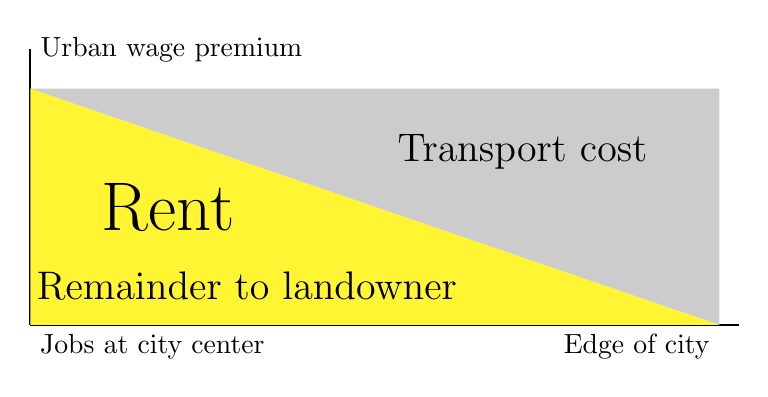
\begin{tikzpicture}[domain=0:2]
\node at (.25,0) [below right, text width=4cm, black ]{Jobs at city center};
% \node at (.25,-1.) [below right, text width=4cm, black ]{center };
% \node at (.25,-2) [below right, text width=4cm, black ]{\Huge Market};
\draw[thick ] (9.25,0)  -- (.25,0);

\draw[thick ] (.25,0)  -- (.25, 3.5)node[ right ]{Urban wage premium};
\fill[yellow!80]  (.25,0) --(.25,3)--(9,0)node[below left, black]{ Edge of city} --cycle;
\fill[gray!40] (9,3) --(.25,3)--(9,0) --cycle;

\node  at (2.,1.5)[font=\Huge ]{Rent};
\node  at (3,.5)[font=\Large]{ Remainder to landowner};
\node  at (6.5,2.2){\Large Transport cost};
% \draw[latex-, line width=1.5mm] (9,-.25) --(9, -2);
% \draw[-latex, line width=.75mm] (.25,-4)node[above]{distance from centre} --(6,-4);
\end{tikzpicture}

%  \begin{tikzpicture}
% %\node at (.25,0) [below right, black, align=right, red ]{ City center};
% %\node at (-.25,-1) [below left, text width=4cm, black , align=right]{\Huge  };

% \fill[yellow!80]  (.25,0) --(.25,3)--(9,0) --cycle;
% \fill[gray!20] (9,3) --(.25,3)--(9,0) --cycle;

% \node at (9.5,0)[below left, text width=2cm, black, align=right]{ Edge of city};
% % \node at (.25,0) [below right, text width=4cm, black ]{Jobs at city center};
% \node at (-.25,0) [below right, align=left]{Jobs at city center};
% \node at (.25, 3.5)[right]{Urban wage premium};

% \node  at (2.2,1.5)[font=\Huge ]{Rent};
% \node  at (3,.5)[font=\Large]{Remainder to landowner};
% \node  at (6.5,2.2)[font=\Large]{ Transport cost};

% \draw[thick ] (9.25,0)--(.25,0);
% \draw[thick ] (.25,0)--(.25, 3.5);
% \end{tikzpicture} 
\end{centering}
\end{frame}

\note[itemize]{
\item Only the axis labels need to be changed for this figure 
\item The agricultural rice at the center becomes the wage premium at the center.
\item The agricultural market at the center becomes the wage premium job market at the center.
\item Ricardo's extensive margin, the geographical edge of cultivation becomes the edge of the city.}


%%%%%%%%%%%%%%%%%%%%%%%%%%%%%%%%%%%%%%%%%
% \begin{frame}{Urban Rent Theory}
% \begin{itemize}\Large
%     \item The urban theorists developed a model that is isomorphic with respect to travel costs and distance
%     \item \textbf{Workers}  pay to transport \textbf{themselves} to \textbf{jobs} at the center
%     \item They did not explain production or distribution
%     \item     The surplus must still go to landowners as locational rent
%     \item I add the distribution of rents to the urban model landowners to my version of the model
% \end{itemize}
% \end{frame}


%%%%%%%%%%%%%%%%%%%%%%%%%%%%%%%%%%%%%%%%%
\begin{frame}{Ricardo's agricultural rents vs \\Alonso's urban locational rents}
%\begin{figure}[!ht]
\centering
\resizebox{1.05\textwidth}{!}{ 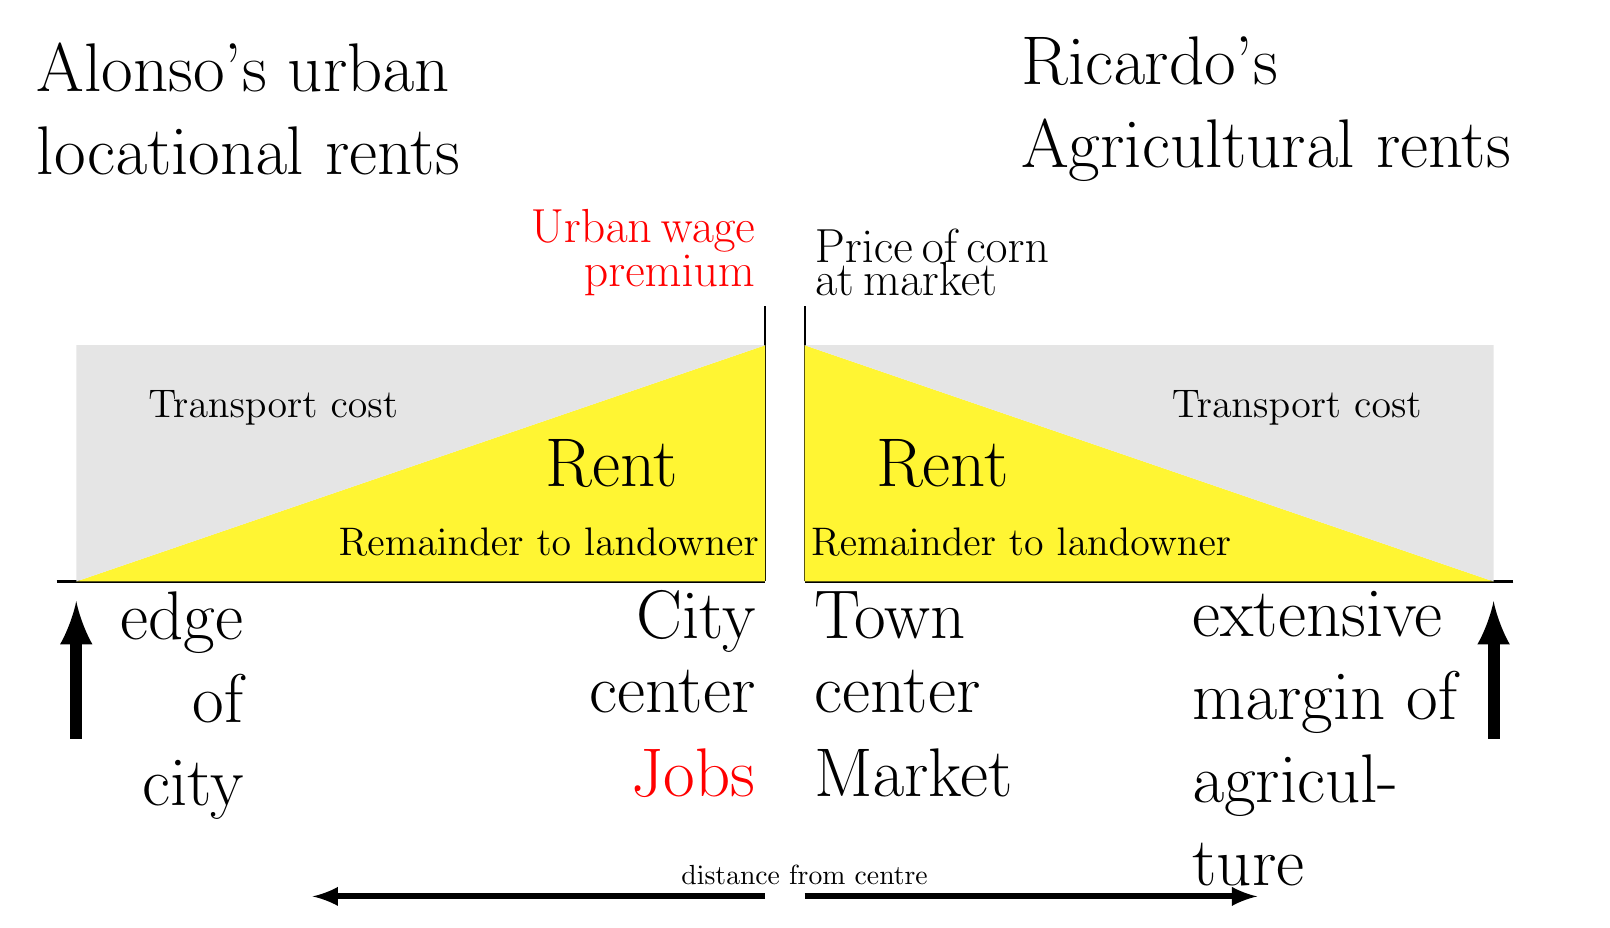
\begin{tikzpicture}[domain=0:2]
 %Combining two RENT figures for one slide
 
%\draw[thick,color=gray,step=.5cm, dashed] (-0.5,-.5) grid (3,3);
%\draw[line width=.01, green ] (0,0) -- (10,0) node[right  ] {Distance};laboutr market
\node at (6.5, 6.) [text width=7cm, font=\Huge ]{Ricardo's\\ Agricultural rents};

\node at (.25,0) [below right, text width=4cm, black ]{\Huge Town };
\node at (.25,-1.) [below right, text width=4cm, black ]{\Huge center };
\node at (.25,-2) [below right, text width=4cm, black ]{\Huge Market};
\draw[thick ] (9.25,0)  -- (.25,0);

\draw[thick ] (.25,0)  -- (.25, 3.5)node[above right, text width=3cm, ]{\LARGE Price of corn at market};
\fill[yellow!80]  (.25,0) --(.25,3)--(9,0)node[below left, black, text width=3.7cm, font=\Huge]{ extensive margin of agriculture} --cycle;
\fill[gray!20] (9,3) --(.25,3)--(9,0) --cycle;

\node  at (2.,1.5)[font=\Huge ]{Rent};
\node  at (3,.5)[font=\Large]{ Remainder to landowner};
\node  at (6.5,2.2){\Large Transport cost};
\draw[latex-, line width=1.5mm] (9,-.25) --(9, -2);
\draw[-latex, line width=.75mm] (.25,-4)node[above]{distance from centre} --(6,-4);

%\pause

%  ALONSO CITY. negative x]

\node at (-6,6.)[text width=7cm, align=left, font=\Huge ]{ Alonso's  urban \\ locational rents};

\node at (-.25,0) [below left, text width=4cm, black, align=right ]{\Huge City };
\node at (-.25,-1) [below left, text width=4cm, black , align=right]{\Huge center };
\node at (-.25,-2) [below left, text width=4cm, red , align=right]{\Huge Jobs};

\draw[thick ] (-9.25,0)  -- (-.25,0);
\draw[thick ] (-.25,0)  -- (-.25, 3.5)node[above left, text width=3cm, align=right, red]{\LARGE Urban wage premium};
\fill[yellow!80]  (-.25,0) --(-.25,3)--(-9,0)node[below right, text width=2cm, black, align=right, font=\Huge ]{ edge of city} --cycle;
\fill[gray!20] (-9,3) --(-.25,3)--(-9,0) --cycle;

\node  at (-2.2,1.5)[font=\Huge ]{Rent};
\node  at (-3,.5)[font=\Large]{ Remainder to landowner};

\node  at (-6.5,2.2){\Large Transport cost};
\draw[latex-, line width=1.5mm] (-9,-.25) --(-9, -2);

\draw[-latex, line width=.75mm] (-.25,-4)--(-6,-4);

\end{tikzpicture} }
\label{fig:Rent_Ricardo_Alonso}
%\end{figure}
\end{frame}


\note[enumerate]{
    \item I am illustrating the two theories to show they are really the same theory 
    \item the isomorphism should lead us to think about who gets the rents
    \item that is basically what  do 
    \item but I also add a production sector that explains where the rents come from
    \item This forces us to pull some ideas from growth and agglomeration theories
 }

%%%%%%%%%%%%%%%%%%%%%%%%%%%%%%%%%%%%%%%%%
\begin{frame}{Later in the 19th century, neoclassical theory described  an industrial society}
\begin{itemize}
\item Economic theory shifted to focusing on production with produced capital instead of natural capital

% \item Space and land no longer played the central role in production

\item Removing the land removed the role of space in the theory of distribution.

\item Workers got the marginal value of their contribution to output and the surplus went to the owners of capital in the form of profit. 

\end{itemize}
\end{frame}


%%%%%%%%%%%%%%%%%%%%%%%%%%%%%%%%%%%%%%%%%
\begin{frame}{Extending the urban model}
\begin{itemize}\Large
    \item They did not explain production or distribution
    \item     The surplus must still go to landowners as locational rent
    \item I add the distribution of rents to the urban model landowners to my version of the model
\end{itemize}
\end{frame}


%%%%%%%%%%%%%%%%%%%%%%%%%%%%%%%%%%%%%%%%%
{    %. the whole frame is enclosed
\usebackgroundtemplate{
\tikz[overlay,remember picture] \node[opacity=0.3, at=(current page.center)]
   {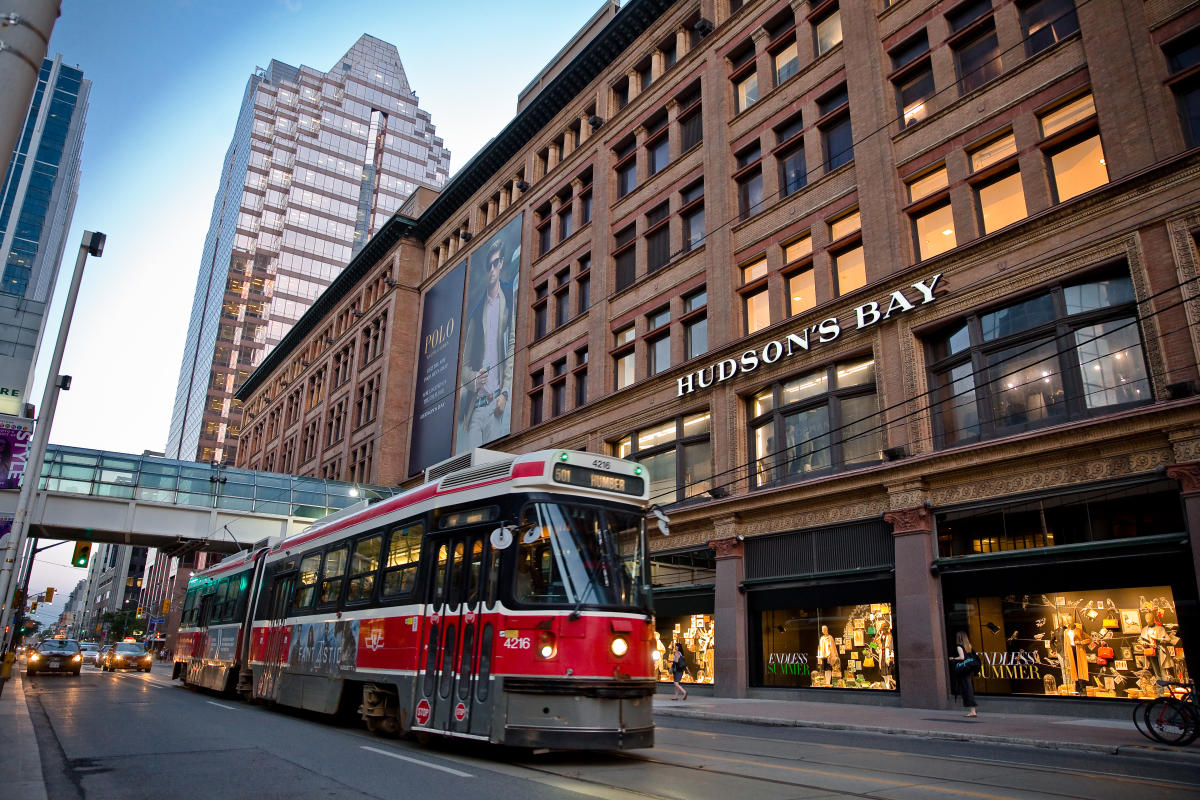
\includegraphics[width=\paperwidth, height=\paperheight]{Toronto.jpg}}
; %end tikz command
} %end background inclusion

\begin{frame}{INTRO TO SCALE - E.G.}



\color{orange!50!black} % textcolor

%\contour{black}{\protect\textcolor{yellow}  {
\Large 
``Cities are the crucible of civilization, the hubs of innovation, .. the magnets that attract creative individuals, and the stimulant for ideas, growth, and innovation'' %}}

\vspace{-0.3cm}\hfill Geoffrey West

\hspace{4cm}yet
\vspace{.2cm}

"land is always far cheaper outside cities than inside. .. If we postulate only the usual list of economic forces, cities should fly apart.”

\hfill Robert E. Lucas Jr.

\end{frame}
} % end region background is operating


%%%%%%%%%%%%%%%%%%%%%%%%%%%%%%%%%%%%%%%%%
\begin{frame}{Scaling of total wages}
\begin{tikzpicture}
 \node at (-4,4){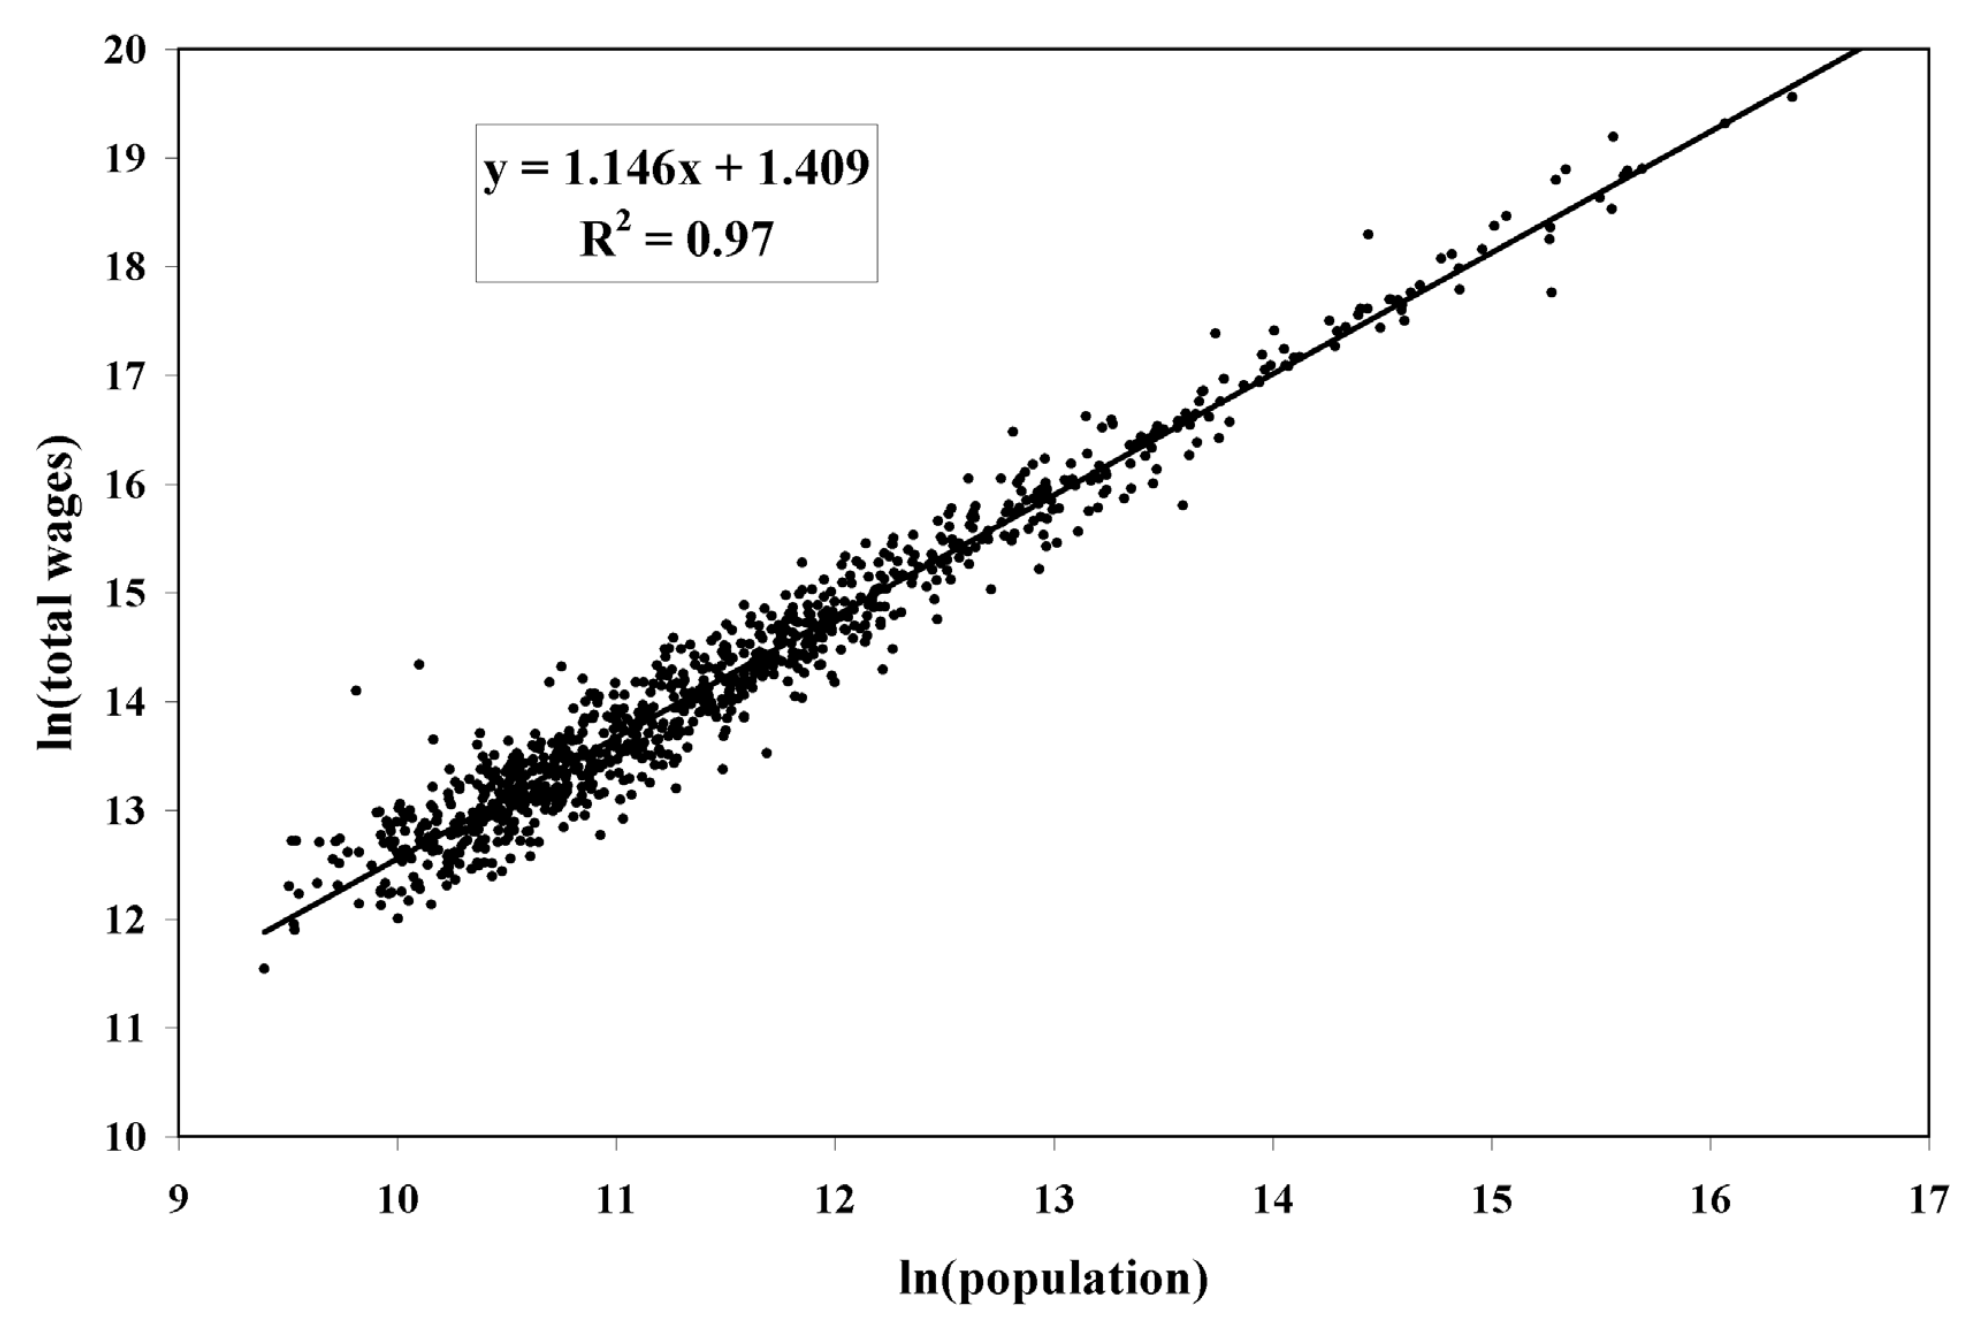
\includegraphics[scale=.3]{ScalingWagesUSA.png}};
%\node at (-4,4){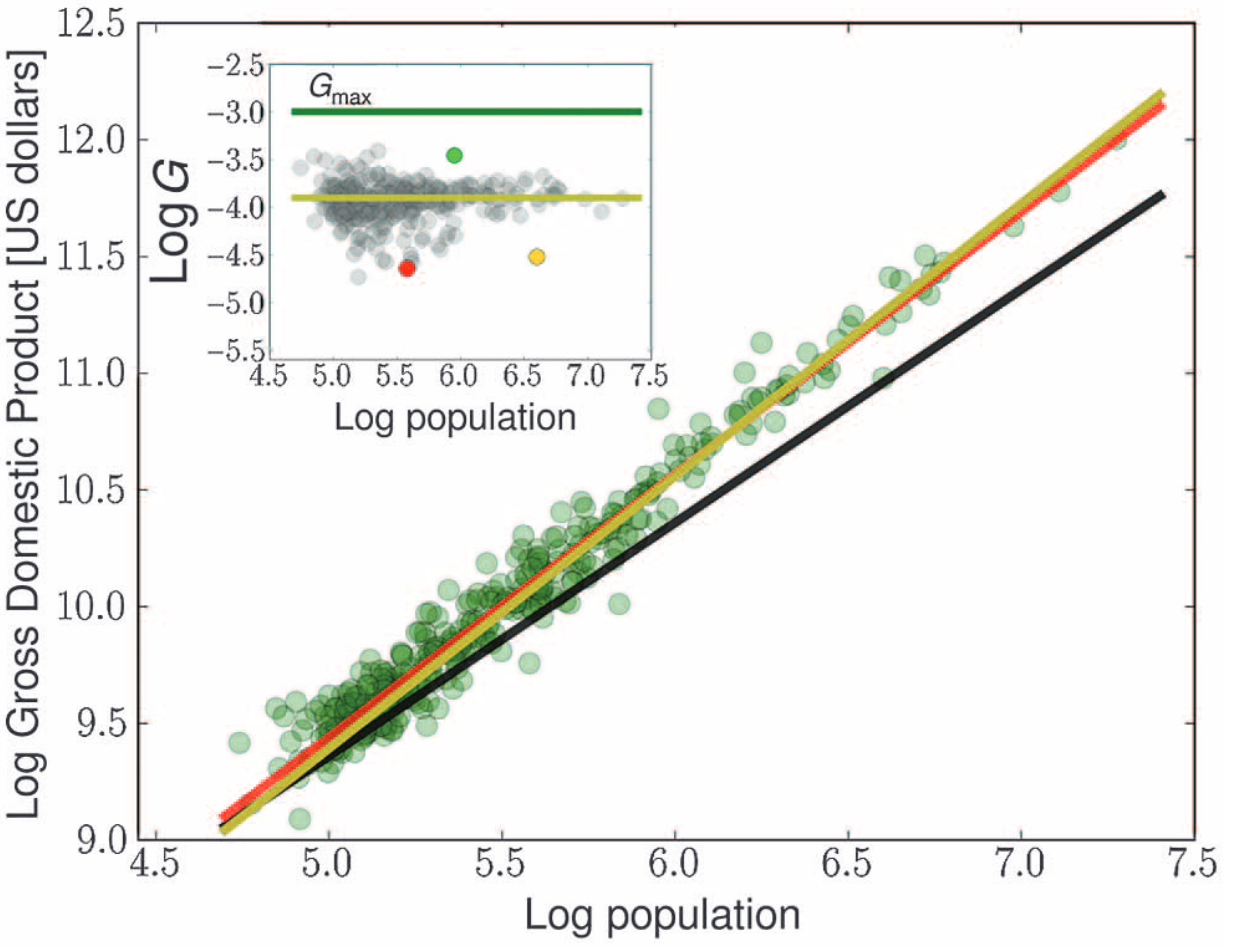
\includegraphics[scale=.3]{ScalingGDP.png}};
\node at (-5.8,5.5){\Large$\beta = 1.146$};
\end{tikzpicture}

\vspace{-.3cm}
\small Scaling of total wages using data for all 943 urban areas of the United States (2009–2011) showing superlinear scaling.

\vspace{.1cm}
\tiny Source: Urban Scaling and the Production Function for Cities. Lobo, Bettencourt, Strumsky, West
\end{frame}

%%%%%%%%%%%%%%%%%%%%%%%%%%%%%%%%%%%%%%%%%
%\usebackgroundtemplate{\includegraphics[width=\paperwidth]{}}
% \begin{frame}{Physiocrats}

%     % \centering
%     % 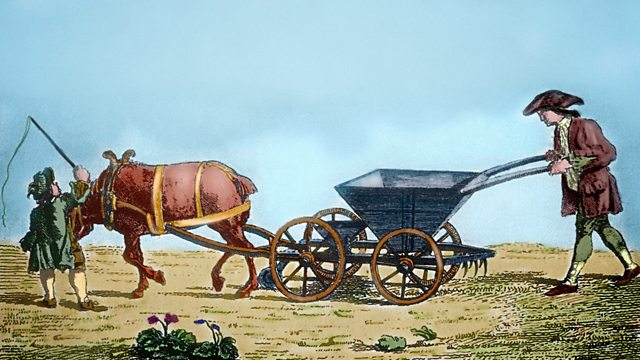
\includegraphics[scale=0.6]{fig/carter_illustration.jpg}
%     % \vspace{-1.5em} % Adjust the vertical space as needed
%     % \begin{flushright}
%     %     \tiny{Source: https://www.bbc.co.uk/programmes/b02x97k6} % braggPhysiocrats2013
%     % \end{flushright}
% \end{frame}



% \begin{frame}{Financialization}
%     \centering
%     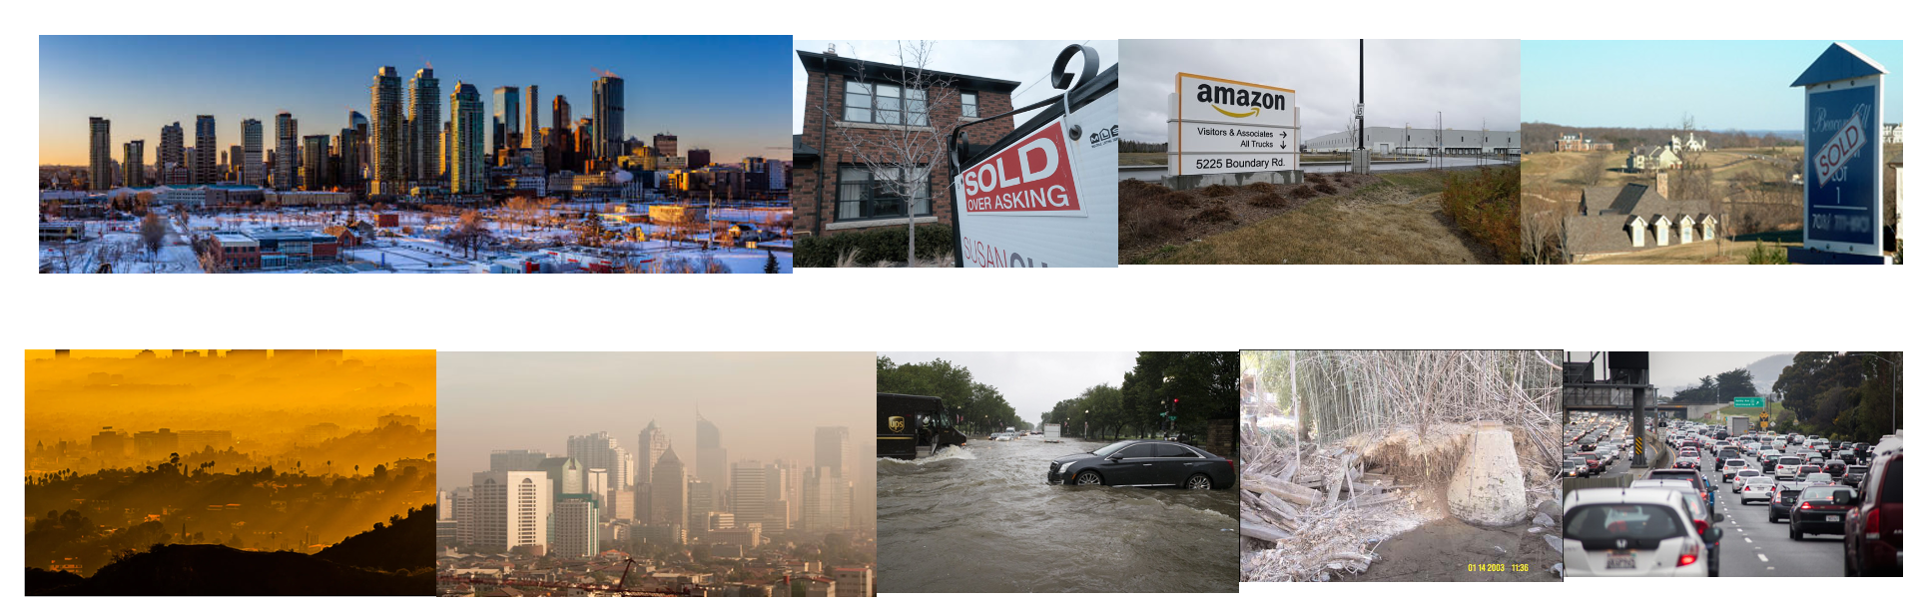
\includegraphics[scale=0.167]{fig/example_figures/pictures-ex-1.png}
%     \vspace{-2.5em} % Adjust the vertical space as needed
%     \begin{flushright}
%         \tiny{Source: Dawn Parker}
%     \end{flushright}
% \end{frame}

%%%%%%%%%%%%%%%%%%%%%%%%%%%%%%%%%%%%%%%%%
\begin{frame}{Increasing returns in the city}

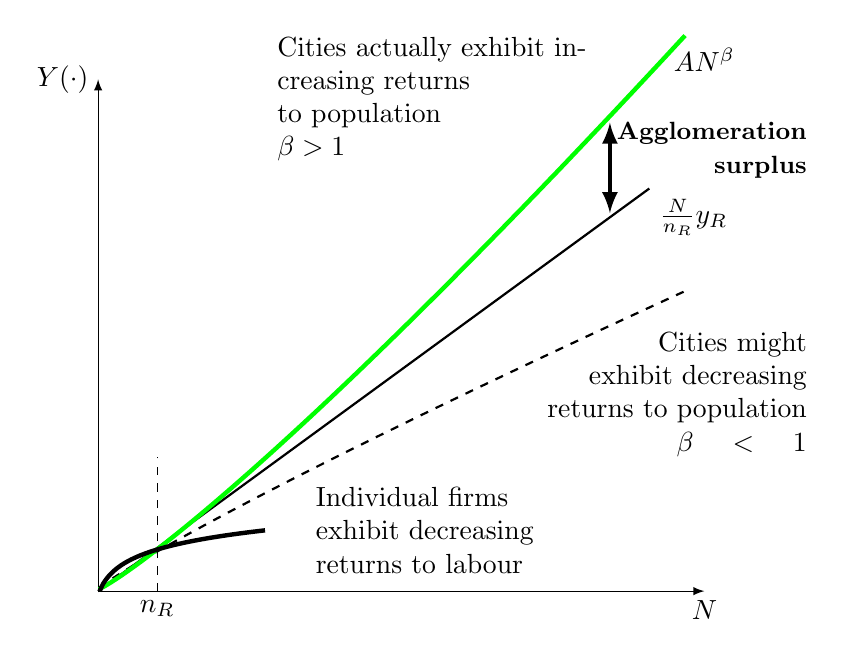
\begin{tikzpicture}[scale=.5, my plot/.style={thick, smooth, samples=100, domain=0.1:2.2},
plot2/.style={thick, smooth, samples=100, domain=0.1:14.99},
                    my grid/.style={dashed,opacity=0.5, every node/.style={black,opacity=1}},
                    my axis/.style={latex-latex}]
 
 \draw[my axis] (0,13)node[left] {$Y(\cdot)$} --(0,0)-- (15.4, 0) node[below] {$N$}; %creates the axis a little 

\coordinate (origin) at (0,0);
\def\x{0.45}
\def\y{2.1}
\def\b {$15/(2*ln(\y)+.05)$};
%\def\p{0.55} % define the x, y and p )(midpointvalues
%\draw[my plot] (0,0) plot (\x,{ln(\x)});  %Draws curve
%\draw[my plot] (0,0) plot ({\x-.08},{2.3+ln(\x)}); 
\coordinate (Uy) at (\y,{2*ln(\y)+.05});

% THREE SCALE POSSIBILITIES
\draw [thick, ](0,0)--(14, 10.22583)node[below right]{$\frac{N}{n_R}y_R$};   %diagonal line CRS
\draw[plot2, dashed] (0,0) plot ({\x-.08},{(\x)^0.9/1.5 }); %DRS
\draw[plot2, ultra thick, green] (0,0) plot ({\x-.08},{(\x/1.5)^1.15});%
\node at (15.4, 13.5){$AN^\beta$};

%  TEXT
\node at (13.8,12.5) [left, text width=4.5cm]{ Cities actually exhibit increasing returns\\ to population\\ $\beta>1$};%IRS
\node at (13.5,5)[text width=4.5cm, align=right] {Cities might\\ exhibit decreasing \\returns to population \\ $\beta<1$};% DRS

% ARROW
\draw[latex-latex, ultra thick] (13, 11.9)--(13, 9.6);
\node at (15.5, 11.2)[ text width=2.5cm, align=right]{\small\textbf{Agglomeration\\ surplus}};

\begin{scope}[ yscale=1,xscale=2]% shift={(1.9,0)} ,
	\coordinate (Uy) at (\y, {2.3+ln(\y)});
  \draw[my plot,ultra thick] (0,0) plot ({\x-.08},{1.15+ln(\x)/2})node[right=.5cm, text width=3.9cm]{Individual firms\\ exhibit decreasing\\ returns to labour}; % production function for generic ferm
	\draw[dashed](.75, 0)node[below]{$n_R$} --(.75, 3.4);
\end{scope}
\end{tikzpicture}
\end{frame}

\note[enumerate]{
    \item just to be clear about what is happening
    \item I have a little decreasing returns to scale firm down here in the corner. (Equation 2)
    \item I can add a lot of them all at optimal scale to get a CRS city. That is the black straight line 
    \item but the city might get crowded or be expensive to operate, so the city as a whole should exhibit DRS -  dashed line
    \item The fact is *(Jacobs, Scale lit) they exhibit IRS. Green line. (Equation 1)this is what we have to build in with agglomeration economies in equation 3
}


%%%%%%%%%%%%%%%%%%%%%%%%%%%%%%%%%%%%%%%%%



\begin{frame}{Formally modelling production and growth with DRS firms and IRS cities}
% - TODO FIX SUBSCRIPT AND HIGHLIGHT }%{Production and the city}
\Large 
1) $Y=AN^\beta$ {\normalsize \hfill \textbf{Scale literature and Jacobs}\\\hfill $N =$ population}
\vspace{.5cm}

2) $y=A^{firm} k^\alpha n^{\beta_{firm}}$ \  \hfill{\normalsize \textbf{Neoclassical production function}\\\hfill $n =$ firm workforce}
% 2) $y=\:A\" \;k^\alpha n^\beta$ {\normalsize \hfill \textbf{Neoclassical production\\ 
% \hfill function}\\ 
% \hfill$n =$ {{\normalsize firm workforce}
\vspace{.5cm}

 \color{red}3) $y=A^{firm}N^\gamma k^\alpha n^{\beta_{firm}}$ {\normalsize \hfill \textbf{Synthesis in our model}\\ \hfill $N = F n, \qquad F=$ number of firms}

% $Y= FA^{firm}F^\gamma n^\gamma z^\alpha n^\alpha n^{\beta_{firm}} = A(Fn)^{\gamma+\alpha +\beta_{firm}}$ where $A=A^{firm}F^{1-\alpha-\beta}z^\alpha$, and  $k=zn$

\end{frame}

\note[enumerate]{
\item equation 1 has been estimated in the scaling literature.  beta greater than one $\rightarrow$  productivity gets bigger as the population increases.
    
    This says that bringing people together raises everyone’s productivity. IRS 
\item firms a=suppressedin this formulation
    
\item Neoclassical Growth theorists useds  Cobb-Douglas production function. It has
    
    This has diminishing returns at the firm level. According to the theory the wage is the VMPL, so we have a theoretically consistent way to derive the wage
    
\item We can show the two equations are nested in the following
\item    We make the productivity term depend on urban population. If the population rises, wages rise.
    
\item This is now a linked firm-city model of production with DRS for the firm and IRS for the City
\item $Y= FA^{firm}F^\gamma n^\gamma z^\alpha n^\alpha n^{\beta_{firm}}$

$ = A(Fn)^{\gamma+\alpha +\beta_{firm}}$
where $A=A^{firm}F^{1-\alpha-\beta}z^\alpha$, and  $k=zn$)
}

%%%%%%%%%%%%%%%%%%%%%%%%%%%%%%%%%%%%%%%%%
\begin{frame}{}
  \centering \Large
  %\emph
  {The model main loop:}
  
    %\emph
    {three blocks}
  
\end{frame}

% \begin{frame}<1>
%   \frametitle<1>{A Complicated Picture}
%   \framezoom<1><2>[border](0cm,0cm)(2cm,1.5cm)
%   \framezoom<1><3>[border](1cm,3cm)(2cm,1.5cm)
%   \framezoom<1><4>[border](3cm,2cm)(3cm,2cm)
%   \begin{centering}
%         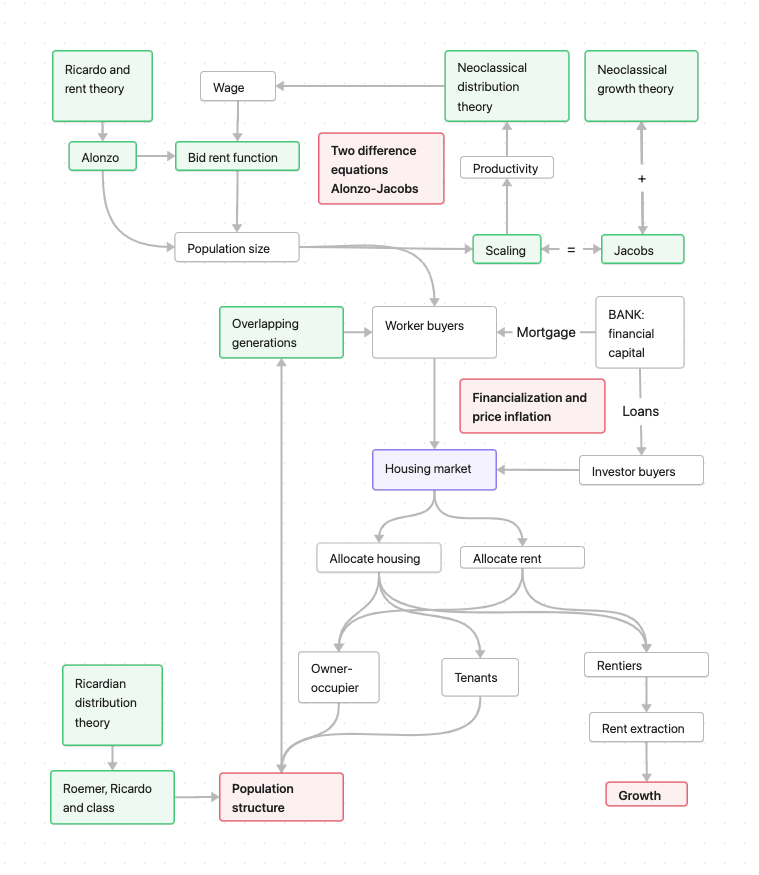
\includegraphics[height=0.95\paperheight]{fig/flow_full_model.png}
%     \end{centering}
% \end{frame}
% \againframe<2->[plain]{zooms}

%%%%%%%%%%%%%%%%%%%%%%%%%%%%%%%%%%%%%%%%%
\begin{frame}{The structure of the model}
    \begin{tikzpicture}
\node at (0,0){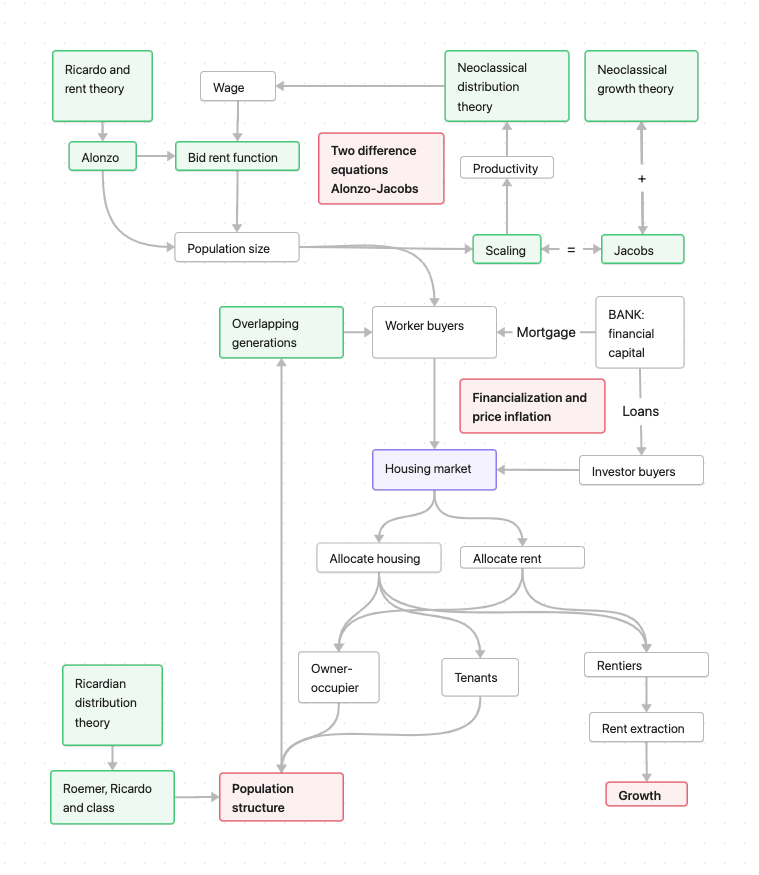
\includegraphics[scale=.07, trim={1cm 1cm 1cm 1cm}, clip]{fig/flow_full_model.png}};

%\only<1>{\draw (3.5,0)rectangle (7,4);}
%\node at (4,0)[text with=2cm,  align= left] {The green boxes around the edges identify where specific theoretical components are inserted. \\The main loop has three min pieces, representing the production side, the finance sector and the housing market,. };
% \draw [step=1,black, thin] (-3,-4) grid  (3,4);
% \draw [step=.25,gray!50, thin] (-3,-4) grid  (3,4);


\only<2>{
\draw[red, line width=1mm] (-2.2, 4)  rectangle (2,1.5);
\node at (5.25, 3.6)[red]{\Large Alonso-Jacobs cycle};
\node at (5.25, 2.1)[text width=3.5cm]{  Wage → \\\:Extent → \\\:\:Population → \\\:\:\:Productivity → \\\:\:\:\:Wage → };
}  %{Alonso Model:   wage → extent → population
% Jacobs Agglomeration: population → productivity 
% Neoclassical Production Function:               productivity → wage }

% \only<3>{
% \draw[green, line width=1mm, fill=yellow!50, opacity=.4](-.5, 1.5) rectangle (3.2,-.7);
% \node at (5.25, 1.5)[red]{\Large Finance/lending};
% \node at (5.25, -.1)[text width=3.5cm]{\textbf{Two seller types}\\retirees, investors\\\textbf{Two buyer types:}\\new workers, investors };
% }

% \only<4>{
% \draw[red, line width=1mm]  (-1.7, 0)  rectangle (3.5, -4);\node at (5.35, -.3)[red]{\Large Housing market};
% \node at (5.5, -1.2)[text width=3.5cm]{Allocates\\ housing and rents };
% }
\end{tikzpicture}

\end{frame}

\note[enumerate]{\item }{}

%%%%%%%%%%%%%%%%%%%%%%%%%%%%%%%%%%%%%%%%%
% \begin{frame}<1-2>[label=zooms]{}
%     \frametitle<1>{The structure of the model}
%     \frametitle<2>{ The Alonzo-Jacobs Cycle }
%     \frametitle<3>{The Financial System}
%     \frametitle<4>{The housing market with three classes}
%     %.         border, title
%     \framezoom<1><2>[border](1.7cm,.4cm)(4.4cm,2.1cm)
%     \framezoom<1><3>[border](3.8cm,3.cm)(3.6cm,2cm)
%     \framezoom<1><4>[border](2.cm,4.5cm)(5.cm,4.3cm)
%     \begin{centering}
%     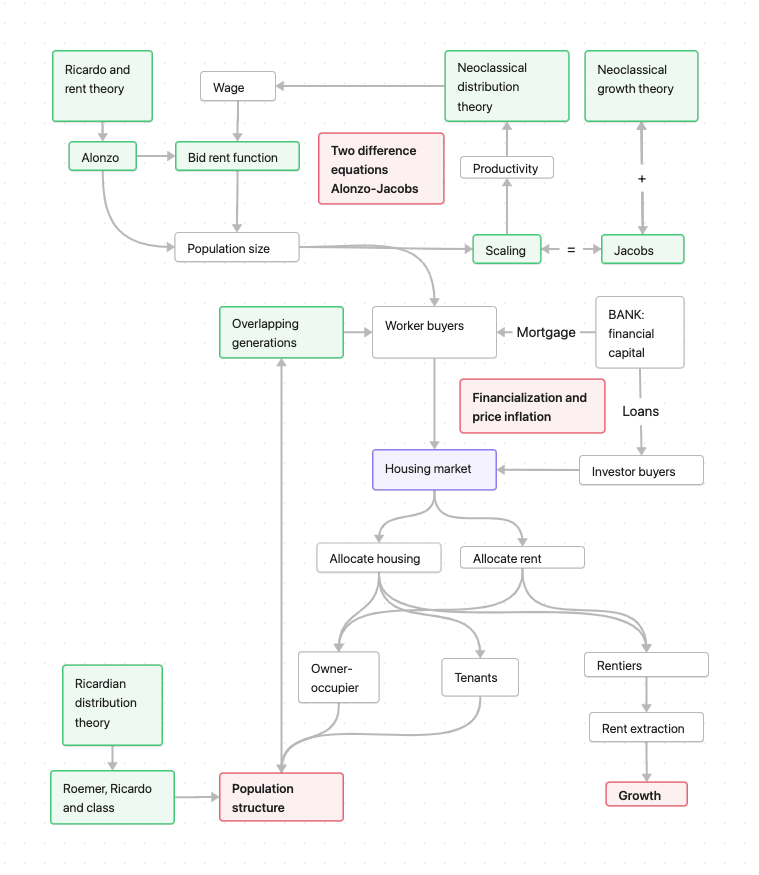
\includegraphics[height=0.95\paperheight]{fig/flow_full_model.png}
%     \end{centering}
% \end{frame}
 
% \againframe<1->[noframenumbering]{zooms}

%%%%%%%%%%%%%%%%%%%%%%%%%%%%%%%%%%%%%%%%%
\begin{frame}{The production system}\framesubtitle{The Alonzo-Jacobs Cycle}
% \begin{figure}[!ht]
\vspace{-.5cm}
\Wider[4em]{\centering
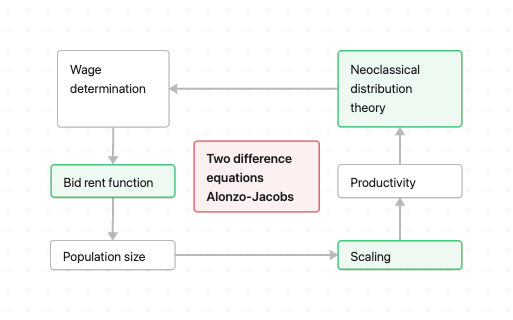
\includegraphics[scale=.55,trim={.5cm 0cm 0 1.cm},clip]{fig/flow-alonso-jacobs-cycle.png}
}
% \caption[Production system.]{The production system component, incorporating the urban scaling of wealth in the urban spatial model. We name this coupling of two difference equations the Alonso-Jacobs cycle.}
% \label{fig-alonso-jacobs-cycle}
% \end{figure}

\vspace{-.5cm}
\hspace{1cm}ALONZO \hspace{5.5cm} JACOBS
\end{frame}


\note[enumerate]{\item This could be modeled as two difference equations 


\item My population adjustment mechanism is actually based on independent decisions by agents, but equation 6 on the next slide captures the effect }

%%%%%%%%%%%%%%%%%%%%%%%%%%%%%%%%%%%%%%%%%
\begin{frame}{Key equations}%The Alonso-Jacobs Cycle: \\\hspace{.5cm}production $\rightarrow$ wage$\rightarrow$population$\rightarrow$production}
\huge 
4) $w=\frac{\beta y} {n}$ {\normalsize \hfill \textbf{Firm behavior}\\\hfill $ w =$ wage}
\vspace{.5cm}

5) $\omega=w-\psi$ {\normalsize \hfill \textbf{Wage premium}\\\hfill $ \psi=$ subsistence wage}
\vspace{.5cm}

6) $N= 2\left[\frac{\omega}{c}\right]^2$ {\normalsize \hfill \textbf{Population equilibrium}\\\hfill $ c=$ transportation cost}

\end{frame}

\note[enumerate]{\item This first equation is just the marginal productivity of workers. It is the derivative of equation 2 with respect to $n$.To maximize profits firms should follow this rule. I assume they do.
\item The second equation just identifies the part of the wage the firm pays that is above the rural wage. In the Alonso model it attracts people to the city
\item The third is a simple calculation of area for a \textbf{city grid}. Agents at the edge of the city decide to work or not, so this is an approximation at any point in time.

(I have left out density to keep it simple)  
} 


%%%%%%%%%%%%%%%%%%%%%%%%%%%%%%%%%%%%%%%%%
\begin{frame}{Financing buyers}
    \begin{tikzpicture}
\node at (0,0){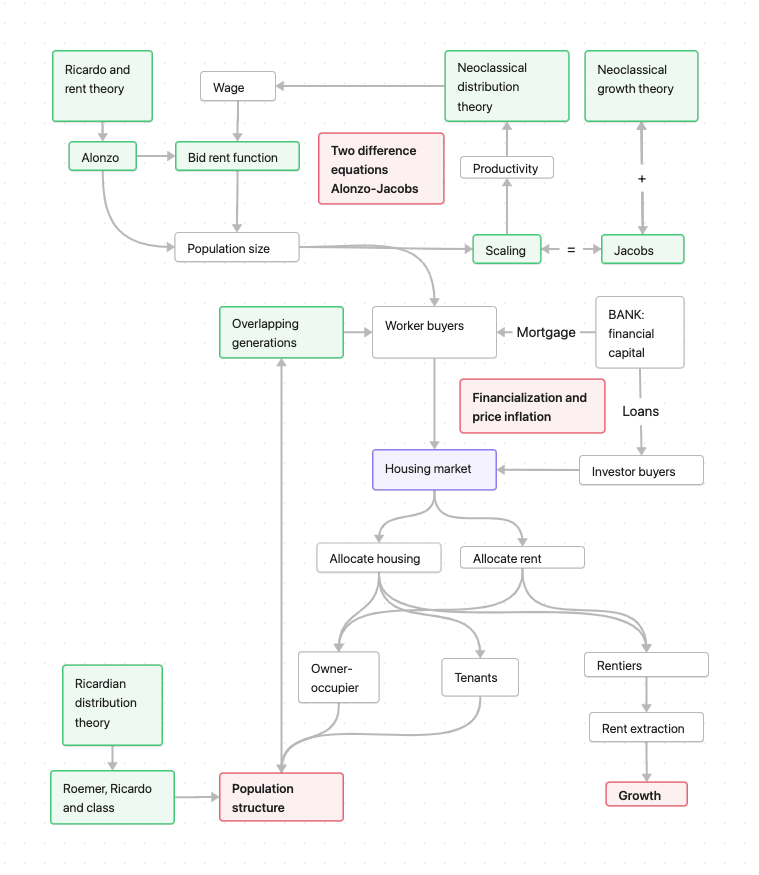
\includegraphics[scale=.07, trim={1cm 1cm 1cm 1cm}, clip]{fig/flow_full_model.png}};

\draw[green, line width=1mm, fill=yellow!50, opacity=.4](-.5, 1.5) rectangle (3.2,-.7);
\node at (5.25, 1.5)[red]{\Large Finance/lending};
\node at (5.25, -.1)[text width=3.5cm]{\textbf{Two seller types}\\retirees, investors\\\textbf{Two buyer types:}\\new workers, investors };
% \only<4>{
% \draw[red, line width=1mm]  (-1.7, 0)  rectangle (3.5, -4);\node at (5.35, -.3)[red]{\Large Housing market};
% \node at (5.5, -1.2)[text width=3.5cm]{Allocates\\ housing and rents };
% }
\end{tikzpicture}
\end{frame}

\note[enumerate]{\item }{}



%%%%%%%%%%%%%%%%%%%%%%%%%%%%%%%%%%%%%%%%%
\begin{frame}{The financialization component}
% \begin{figure}[!ht]
\centering
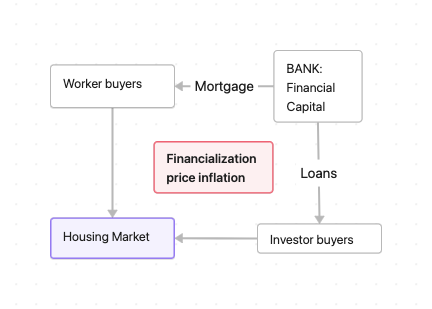
\includegraphics[scale=.175]{fig/flow-financialization.png}
% \caption[The financialization component of the model.]{The financialization component. There is a feedback loop in which new investors drive up demand and thus drive up prices.}
% \label{fig-financial-cycle}
% \end{figure}
\end{frame}



%%%%%%%%%%%%%%%%%%%%%%%%%%%%%%%%%%%%%%%%%
\begin{frame}{The housing market with three classes}
    \begin{tikzpicture}
\node at (0,0){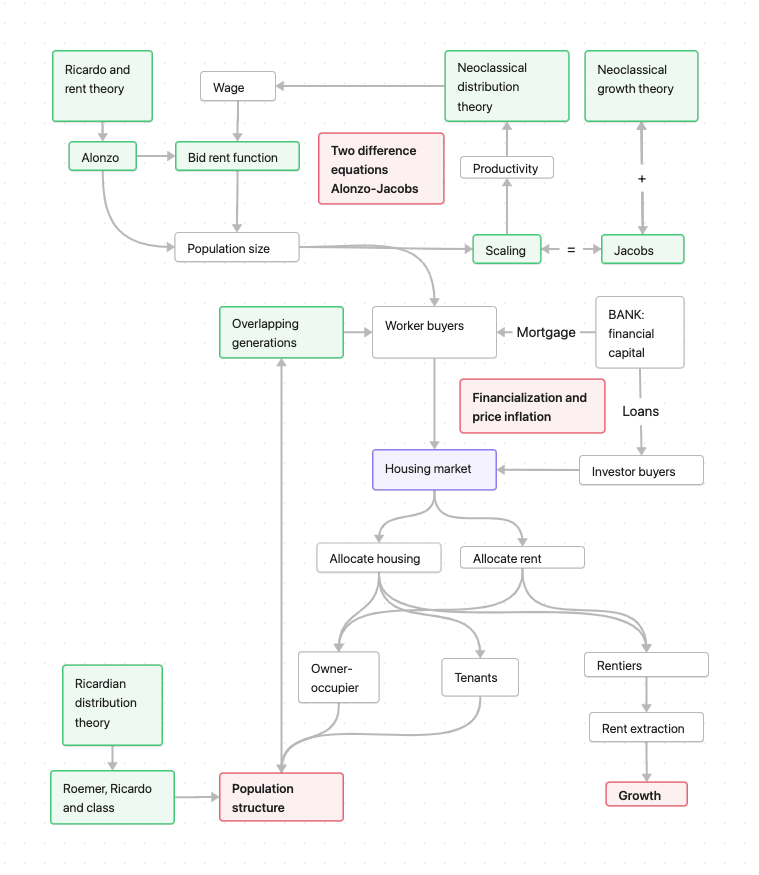
\includegraphics[scale=.07, trim={1cm 1cm 1cm 1cm}, clip]{fig/flow_full_model.png}};

% \only<1>{\draw (3.5,0)rectangle (7,4);}
% \node at (4,0)[text with=2cm,  align= left] {The green boxes around the edges identify where specific theoretical components are inserted. \\The main loop has three min pieces, representing the production side, the finance sector and the housing market,. };
% \draw [step=1,black, thin] (-3,-4) grid  (3,4);
% \draw [step=.25,gray!50, thin] (-3,-4) grid  (3,4);


% \only<2>{
% \draw[red, line width=1mm] (-2.2, 4)  rectangle (2,1.5);
% \node at (5.25, 3.6)[red]{\Large Alonso-Jacobs cycle};
% \node at (5.25, 2.1)[text width=3.5cm]{  Wage → \\\:Extent → \\\:\:Population → \\\:\:\:Productivity → \\\:\:\:\:Wage → };
% }  %{Alonso Model:   wage → extent → population
% Jacobs Agglomeration: population → productivity 
% Neoclassical Production Function:               productivity → wage }

% \only<3>{
% \draw[green, line width=1mm, fill=yellow!50, opacity=.4](-.5, 1.5) rectangle (3.2,-.7);
% \node at (5.25, 1.5)[red]{\Large Finance/lending};
% \node at (5.25, -.1)[text width=3.5cm]{\textbf{Two seller types}\\retirees, investors\\\textbf{Two buyer types:}\\new workers, investors };
% }


\draw[red, line width=1mm]  (-1.7, 0)  rectangle (3.5, -4);\node at (5.35, -.3)[red]{\Large Housing market};
\node at (5.5, -1.2)[text width=3.5cm]{Allocates\\ housing and rents };

\end{tikzpicture}

\end{frame}





%%%%%%%%%%%%%%%%%%%%%%%%%%%%%%%%%%%%%%%%%
\begin{frame}{The housing market with three classes}

\begin{center}
 \vspace{-.5cm}   
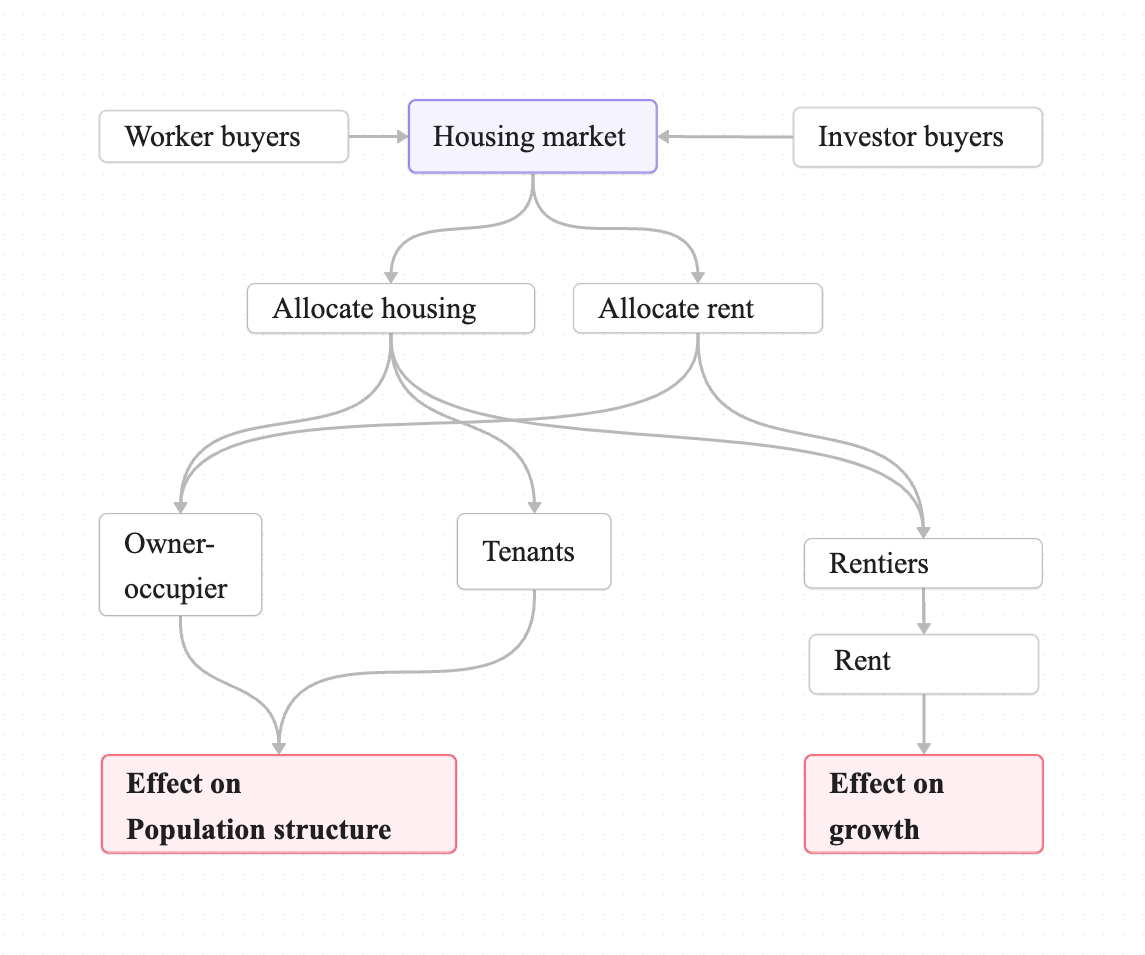
\includegraphics[scale=.14,trim={.5cm 1cm 0 2.5cm},clip]{fig/flow-impacts.png}
\end{center}

% \caption[The housing market component of the model.]{The housing market component. Financialization affects both the allocation of housing and its allocation of rents.}
\end{frame}

%%%%%%%%%%%%%%%%%%%%%%%%%%%%%%%%%%%%%%%%%
% \begin{frame}{The housing model}
% \includegraphics[scale=.09]{fig/flow-
% \end{frame}
% % %----------------------------%



% % %----------------------------%
% \begin{frame}[plain]{The combined model}
% \centering \vspace{-.15cm}
% \resizebox{8.0cm}{!}{%
%   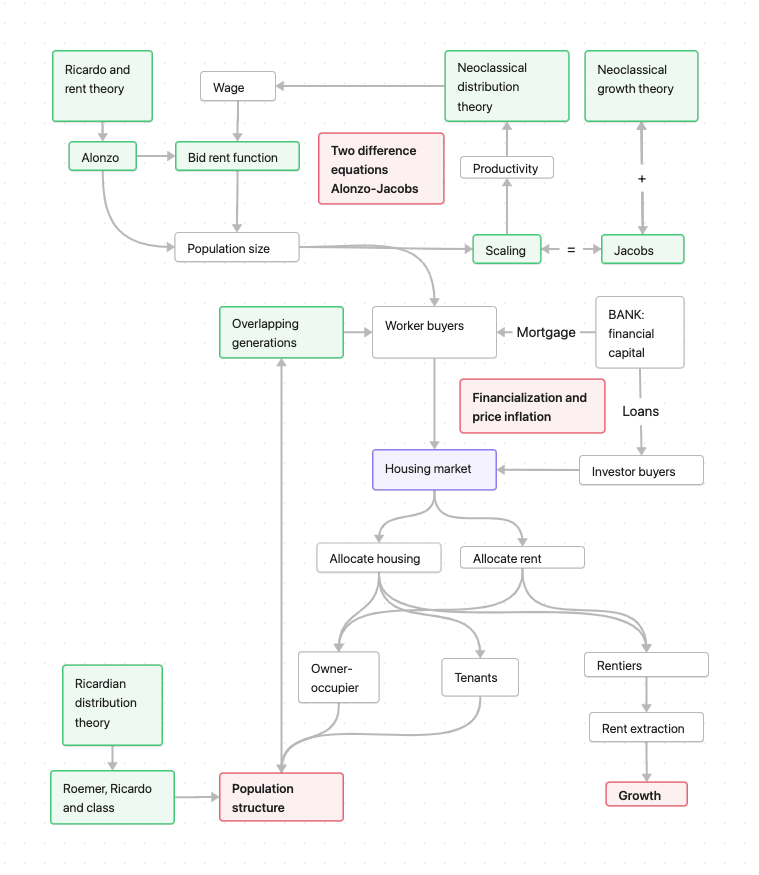
\includegraphics[trim={0cm 0 0 1cm, scale=.5}, clip=]{fig/flow_full_model.png}
%   % \begin{tikzpicture}
%   %   \node at (0,8){The combined model}
%   % \end{tikzpicture}
% }
% \end{frame}

%%%%%%%%%%%%%%%%%%%%%%%%%%%%%%%%%%%%%%%%%
% \begin{frame}{Impact channels relating financialization and urban productivity}
% 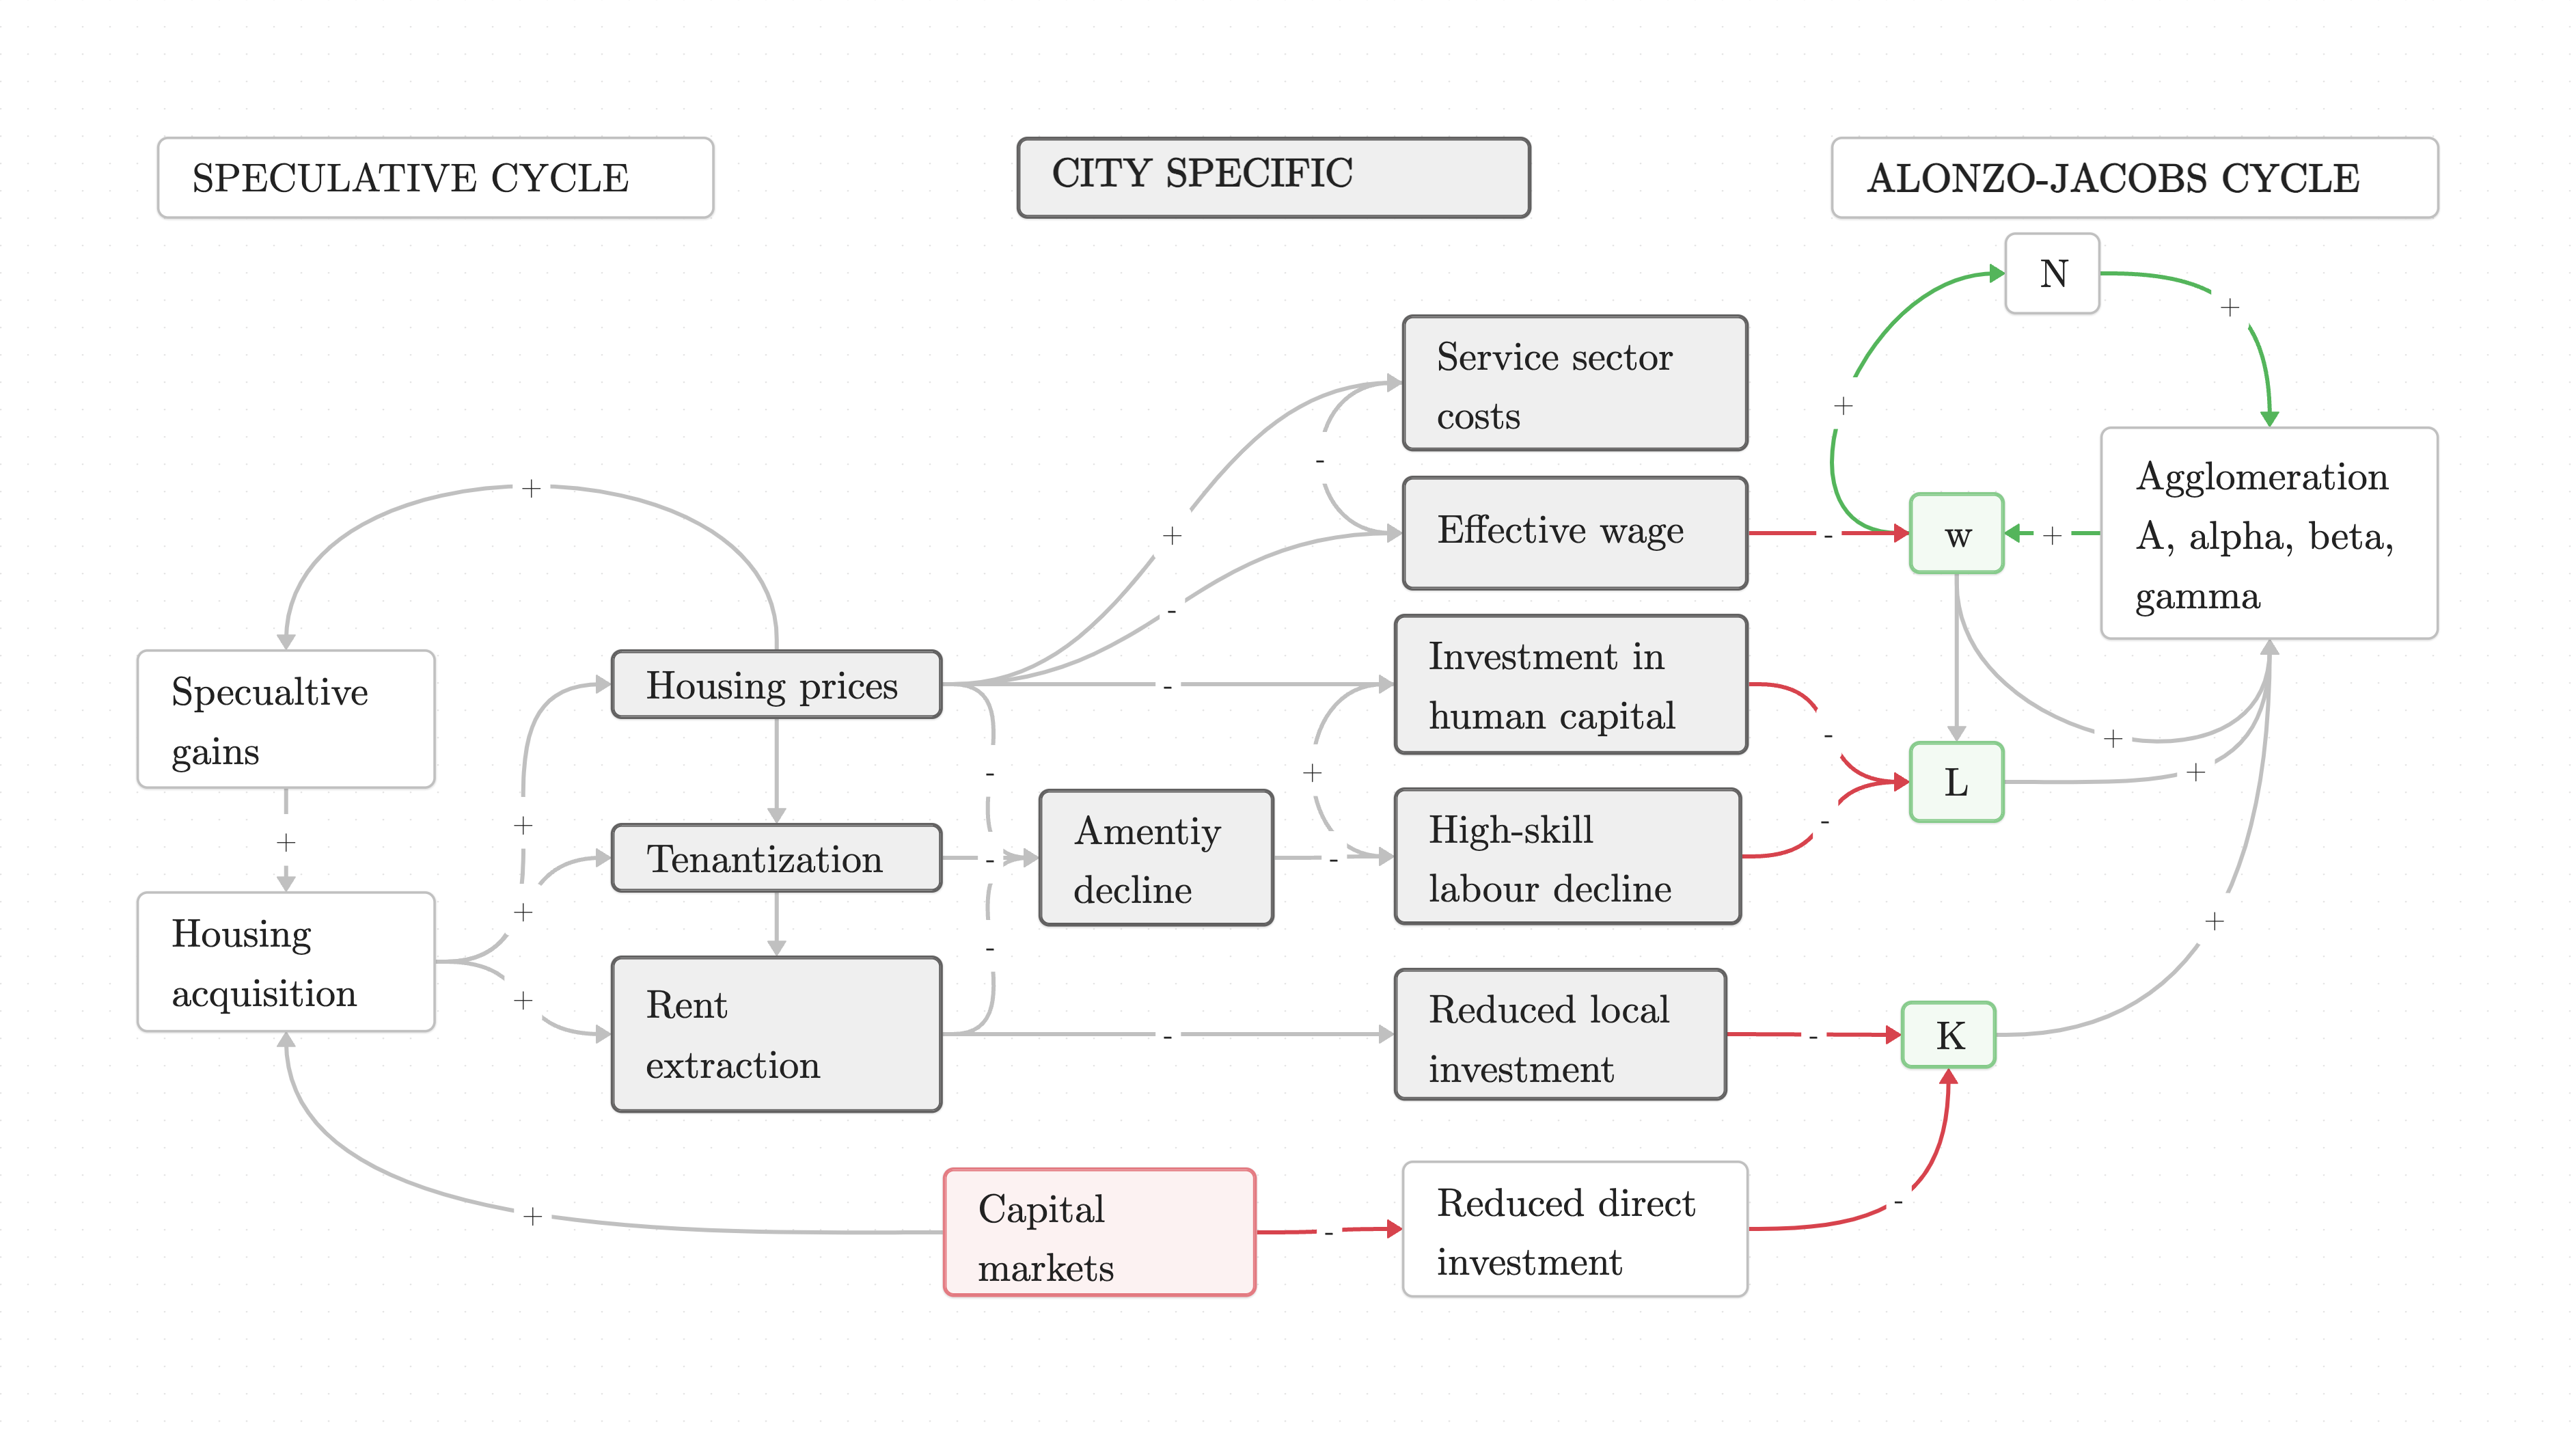
\includegraphics[scale=.09]{fig/impact-channels.png}
% \end{frame}

% %----------------------------%
\begin{frame}{}
%\begin{adjustbox}{max totalsize={1.2\textheight}{.7\textheight},center}
 \centering 
\resizebox{10.0cm}{!}{%
 \centering\vspace{-3cm}
% \tikzstyle{startstop} = [rectangle, rounded corners, minimum width=3cm, minimum height=1cm,text centered, draw=black, fill=red!30]
\tikzstyle{process} = [rectangle, minimum width=3cm, minimum height=1cm, text centered, draw=black, fill=orange!30]
% \tikzstyle{decision} = [rectangle, minimum width=3cm, minimum height=1cm, text centered, draw=black, fill=green!30]
% \tikzstyle{arrow} = [thick,->,>=stealth]


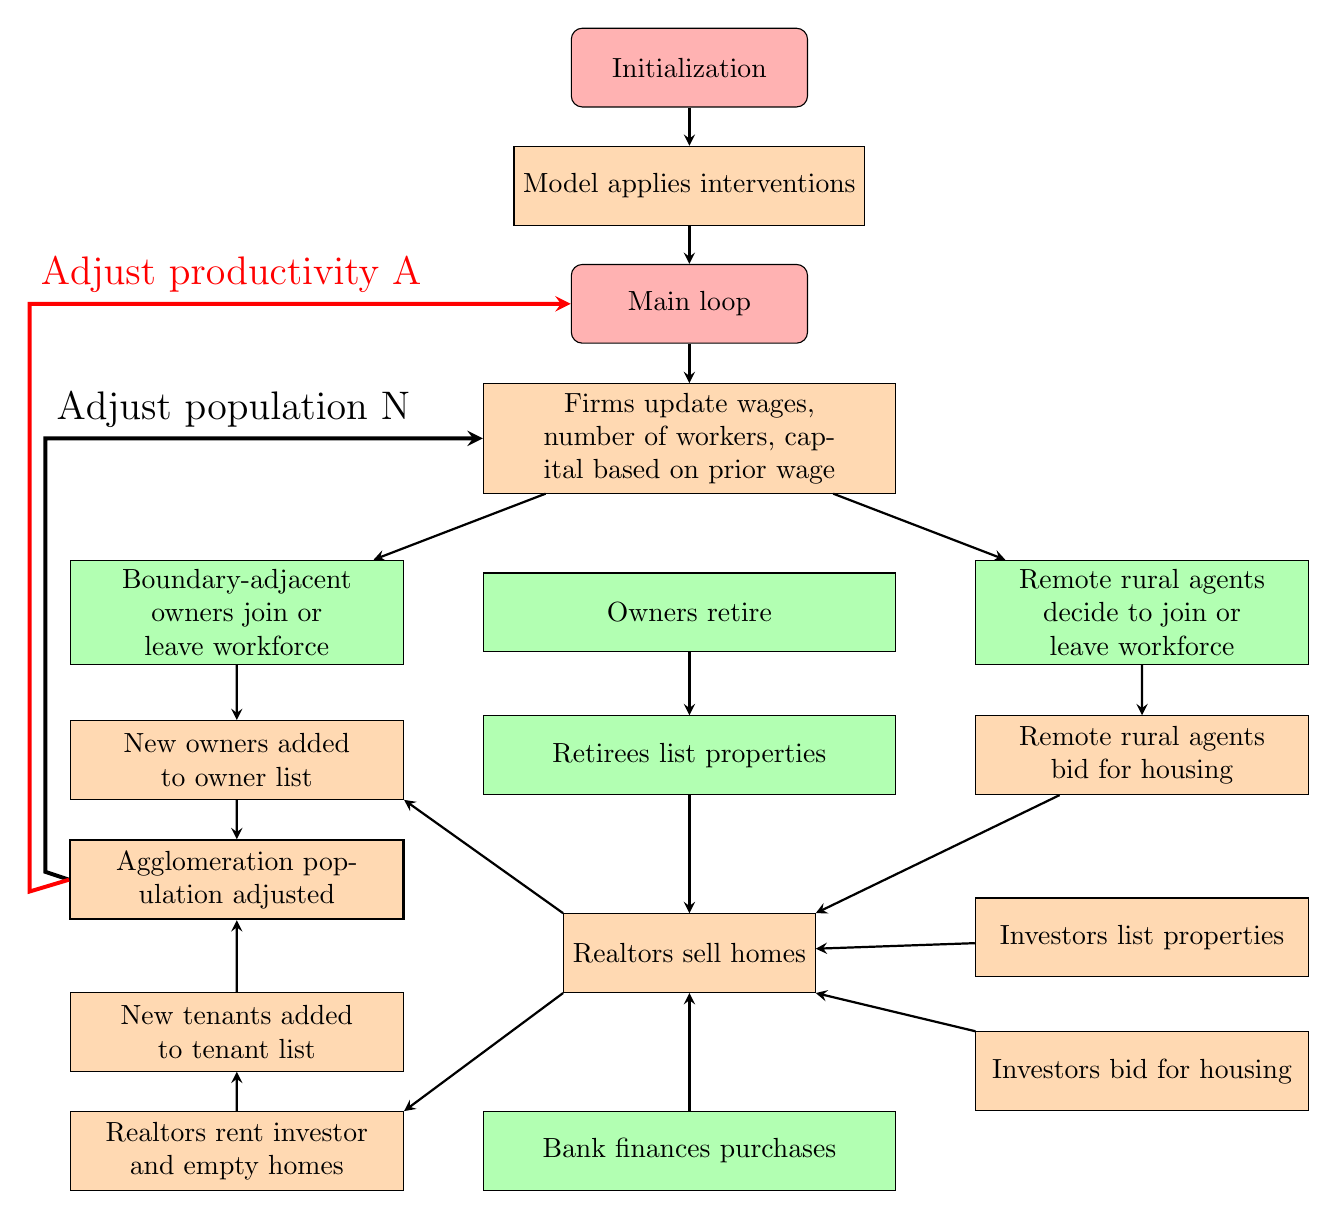
\begin{tikzpicture}[scale=.2,node distance=1.5cm]
\node (init) [startstop] {Initialization};
\node (interventions) [process, below of=init] {Model applies interventions};
% \node (record) [process, below of=interventions] {Record ownership share and reset counters};
\node (mainloop) [startstop, below of=interventions] {Main loop};
\node (firmupdate) [process, below=.5cm of mainloop, text width=5cm] {Firms update wages, number of workers, capital  based on prior wage};

    \draw [arrow] (init) -- (interventions);
    \draw [arrow] (interventions) -- (mainloop);
    \draw [arrow] (mainloop) -- (firmupdate);


\node (owners-retire) [decision, below=1cm of firmupdate, text width=5cm] {Owners retire};
\node (rural-boundary) [decision, left= 1cm of  owners-retire,  text width=4cm] {Boundary-adjacent owners  join or leave workforce};
\node (rural-remote) [decision,  right =1cm of owners-retire, text width=4cm] {Remote rural agents decide to join or leave workforce};


    \draw [arrow] (firmupdate) -- (rural-boundary);
    \draw [arrow] (firmupdate) -- (rural-remote);

\node (retired-list) [decision, below =.8cm of owners-retire, text width=5cm] {Retirees list properties};
  \draw [arrow] (owners-retire) -- (retired-list);



\node (Remote-bid) [process, right=1cm of retired-list, text width=4cm] {Remote rural agents bid for housing};
 \node (Invest-bid) [process, below=3cm of Remote-bid, text width=4cm] {Investors bid for housing};
    
%\node (invest-list) [process, green, below=6cm of rural-remote, text width=5cm] {investors list properties};land

\node (realtors_sell) [process, below = 1.5cm of retired-list ] {Realtors sell homes};
          \draw [arrow]  (retired-list) -- (realtors_sell);    
          \draw [arrow]  (Remote-bid) -- (realtors_sell.north east);     
\node (invest-list) [process, below=1.3cm of Remote-bid, text width=4cm] {Investors list properties};land
          \draw [arrow]  (invest-list) -- (realtors_sell);      
          \draw [arrow]  (Invest-bid) -- (realtors_sell.south east);               
            
\node (bank) [decision, below = 1.5cm  of realtors_sell, text width=5cm] {Bank  finances purchases};
        \draw [arrow] (bank) -- (realtors_sell);

\node (realtors_rent) [process, left = 1cm of bank, text width=4cm] {Realtors rent investor and empty homes};
        \draw [arrow]  (realtors_sell.south west) -- (realtors_rent.north east)   ; 
        
\node (tenant-adjust) [process, above=.5cm of realtors_rent, text width=4cm] {New tenants added to tenant list};

        \draw [arrow]  (realtors_rent) -- (tenant-adjust)   ;

\node (owner-adjust) [process, below = .7cm of rural-boundary,  text width=4cm] {New owners added to owner list};
  \draw [arrow] (rural-boundary) -- (owner-adjust);
  
\node (agglom-adjust) [process, thick, below = .5cm of owner-adjust, text width=4cm] {Agglomeration population adjusted};


  \draw [arrow] (realtors_sell.north west) -- (owner-adjust.south east);
\draw [arrow] (rural-remote) -- (Remote-bid);
 \draw [arrow] (owner-adjust) -- (agglom-adjust);
\draw [arrow] (tenant-adjust) -- (agglom-adjust);

\draw [arrow, line width=.5mm] (agglom-adjust.west) -- ++(-1.5,.5)  |- (firmupdate)node[midway,above right] {\Large Adjust population N}; 

\draw [arrow, red, line width=.5mm] (agglom-adjust.west) -- ++(-2.5,-.75)  |- (mainloop)node[midway,above right] {\Large Adjust productivity A}; 
%-- ++(0,-.5) -- ++(7,0) |-
%-- ++(0,-.5) -- ++(7,0) |-
% % % Custom arrow path
% % \draw [arrow] ($(advance.south) + (0,-0.5)$) -- ++(0,-1) -- ($(mainloop.south) + (-2,-1)$) -- ($(mainloop.south) + (-2,0)$) -- (mainloop);

\end{tikzpicture}


 }
 %\end{adjustbox}
\end{frame}
\note[enumerate]{\item This is a slightly simplified description of the program flows. (some of the accounting is hidden
\item 4th from the top in the  main loop: Firms set wages hire, buy equipment
\item next three population adjustments happen. On the left,  agents at the edge of the city decide whether to work in the city or not - this adjusts the city size. 
\item in the middle, some workers decide to retire. If they have homes they list them. 
\item  on the right, non-adjacent workers may enter the market and bid for housing 
\item below on the right investor may bid or list their units
\item the bank provides financing  to eligible borrowers
\item on the left, population is updated
\item Adjusted values are fed back}

%%%%%%%%%%%%%%%%%%%%%%%%%%%%%%%%%%%%%%%%%
\begin{frame}{Could financialization affect urban productivity?}
\vspace{-.75cm}\Large Surplus is captured by financial sector
\vspace{.75cm}
\begin{itemize}\Large

\item Surplus may be recycled into additional unproductive speculation
\item Residents may have less to invest in city or businesses
\item Tenants may invest less in human capital
\item Civic investment in amenities might decline, making the city less attractive to skilled labour
\end{itemize}
\end{frame}

%%%%%%%%%%%%%%%%%%%%%%%%%%%%%%%%%%%%%%%%%
\begin{frame}{}
  \centering \Huge
  \emph{Experiments}
\vspace{1cm}

 \Large Seven compound experiments 
 
 2-4 policy settings  
 \vspace{.5cm}

Seven outcome paths 

Two states of the world 
\end{frame}


%\newcommand{\coloruncover}[3]{\temporal<#1>{\colorbox{bg}{\phantom{#3}}}{\colorbox{#2}{\phantom{#3}}}{\colorbox{bg}{#3}}}
%%%%%%%%%%%%%%%%%%%%%%%%%%%%%%%%%%%%%%%%%
\begin{frame}{Seven policy variables}\Large
\begin{enumerate}%\color{red}
\item Investor capital gains tax (CGT)
\item Owner-occupiers capital gains tax
\item The cost of capital%, 
\item Transportation costs%,
\item Urban density%, 
\item Borrower wealth sensitivity%, 
\item The property tax rate%,
\end{enumerate}


\end{frame}% %

% \note[enumerate]{\item I want to emphasize that we are doing comparative dynamics: the outcomes are over 200 time-trajectories.
% \item Let's jump into an example.  }



%%%%%%%%%%%%%%%%%%%%%%%%%%%%%%%%%%%%%%%%%

\begin{frame}{Seven outcome paths, three policy settings}%: 
%\Wider{
\small Capital gains tax for investors, 3 values, no productivity linkage
\begin{tikzpicture} 
\node at (.5cm,10cm){
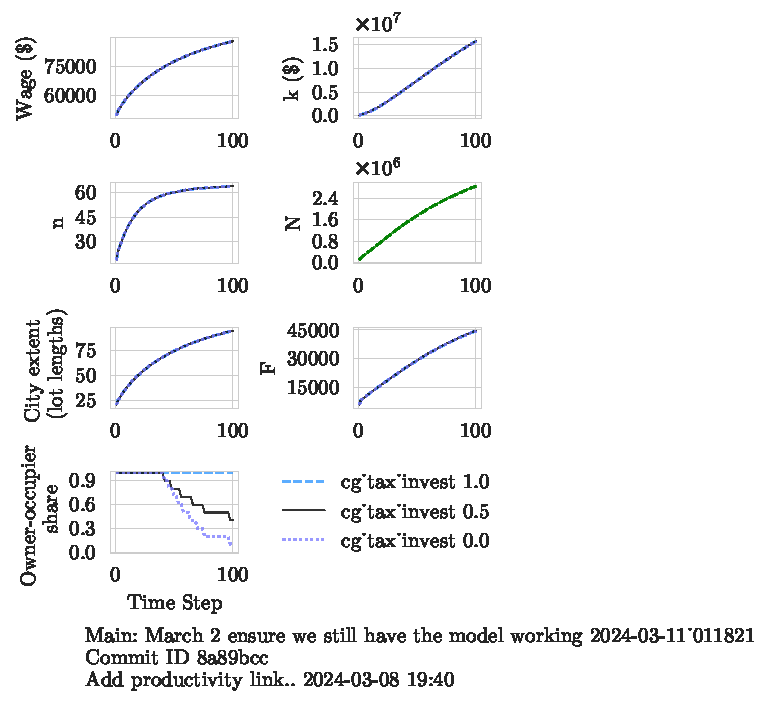
\includegraphics[scale=.75, trim={0 1.4cm 4cm 0},clip]{fig/cg_tax_invest-Main-011821.pdf}};


\node at (6cm,13.35){Wage,\hspace{.4cm} Capital stock};
\node at (6cm,11.5){Workforce,\  Population};
\node at (6.1cm,9.6){City radius,\ \  Number of firms};
\node at (6cm,7.85){Owner-occupier share};

\end{tikzpicture} 
%}
\end{frame}

%%%%%%%%%%
\begin{frame}{Seven policy variables, seven outcome paths}
\Large
\begin{columns}
    \begin{column}{0.5\textwidth}
        \textbf{Seven policy variables}%\coloruncover{1}{yellow!30}{
        \begin{enumerate}
        \item Investor CGT
        \item Owner-occupiers CGT
        \item The cost of capital%, 
        \item Transportation costs%,
        \item Urban density%, 
        \item Wealth sensitivity%, 
        \item The property tax rate%,
    \end{enumerate}
    \end{column}

    \begin{column}{0.5\textwidth}
    \textbf{Seven outcome paths}
    \begin{enumerate}%\color{red}
       \item Wage \item Capital stock\item
       Workforce   \item Population \item City radius \item  Number of firms \item Owner-occupier share
    \end{enumerate}
    \end{column}
\end{columns}
\vspace{.3cm}
\end{frame}% %

%%%%%$%%%%%$%%%%%%%%%$%$%$%%$
\begin{frame}{Capital gains tax on investors with no linkage}
\begin{tikzpicture} 
\node at (.7cm,10cm){
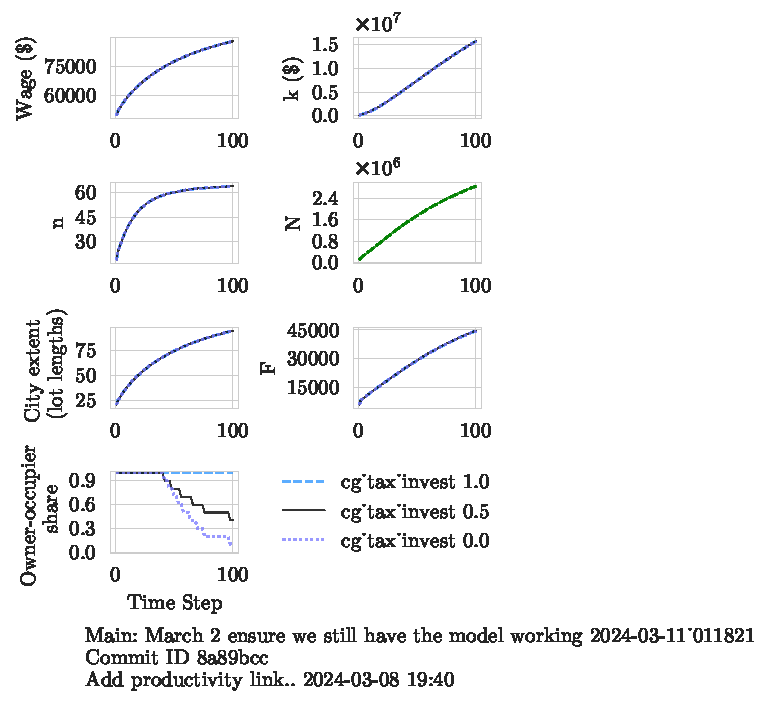
\includegraphics[scale=.8, trim={0 1.4cm 4cm 0},clip]{fig/cg_tax_invest-Main-011821.pdf}};


\node at (6cm,13.5){Wage,\hspace{.4cm} Capital stock};
\node at (6cm,11.56){Workforce,\  Population};
\node at (6.1cm,9.6){City radius,\ \  Number of firms};
\node at (6cm,7.7){Owner-occupier share};

% \pause
% \draw[red!50,line width=1mm] (-.65cm,7.15) ellipse (1.8cm and 1.4cm);
\end{tikzpicture}
\end{frame}

\note[enumerate]{\item This is a set of 3  runs with the base model.
\item The capital gains tax is set at zero 50\% and 100\%

\item This is the no linkage case. Notice that changing the capital gains tax on investors has no effect on `real' variables
\item and the bottom one showing the owner-occupier share of the housing stock. The financial variable affects the rate of financialization.
\item The most significant thing is that a 100\% capital gains tax cuts investor participation to zero, 
\item With no capital gains tax investors eventually take over the entire housing stock. 
\item Do we want to draw policy conclusions from this?
}

%%%%%%%%%%%%%%%%%%%%%%%%%%%%%%%%%%%%%%%%%
\begin{frame}{Adding productivity impacts}
 \centering 
\resizebox{12.5cm}{!}{%
    \begin{tikzpicture}
\node[inner sep=.5pt] (plain) at (0,0)
    {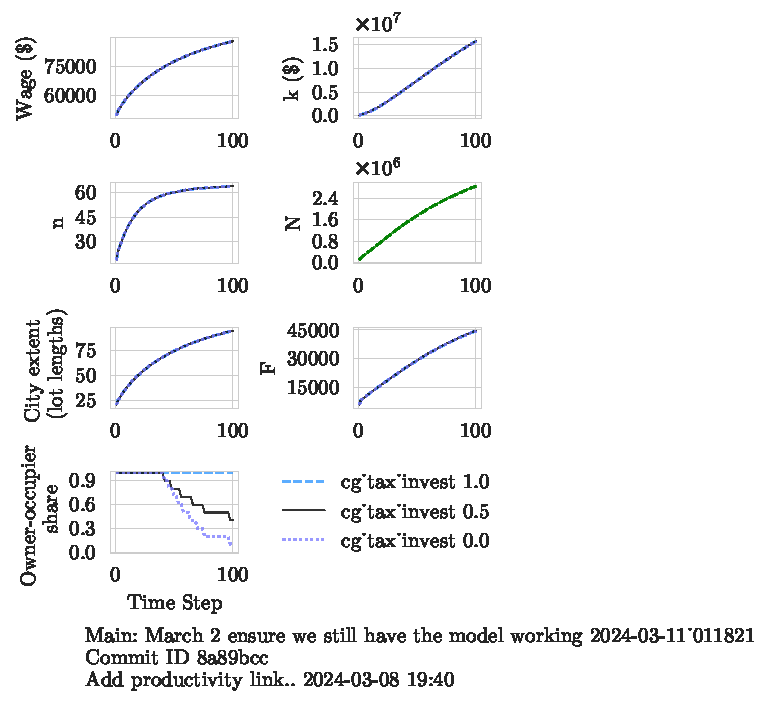
\includegraphics[height=10cm,%width=.5\textwidth,
    trim={.3cm 1.4cm 1cm 0},clip]{fig/cg_tax_invest-Main-011821.pdf}}; 

\node[inner sep=0pt] (link) at (6.8,0)
    {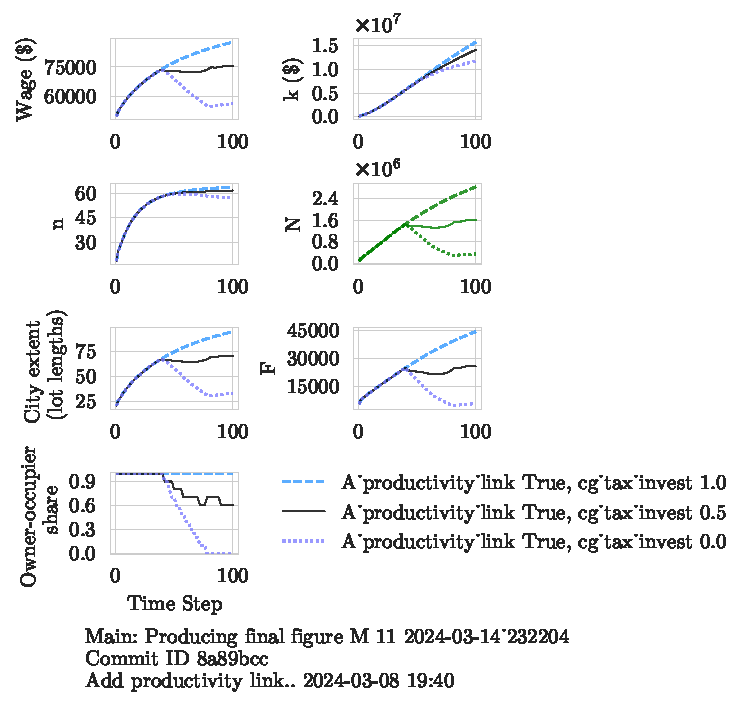
\includegraphics[height=10cm,%width=.5\textwidth, 
    trim={.1cm 1.4cm 4.cm 0},clip]{fig/With-productivity_linkcg_tax_invest-232204.pdf}};
    
\draw[color=white, fill=white] (7,-2.3) rectangle (12.6,-4.5);
\end{tikzpicture}
}
    %  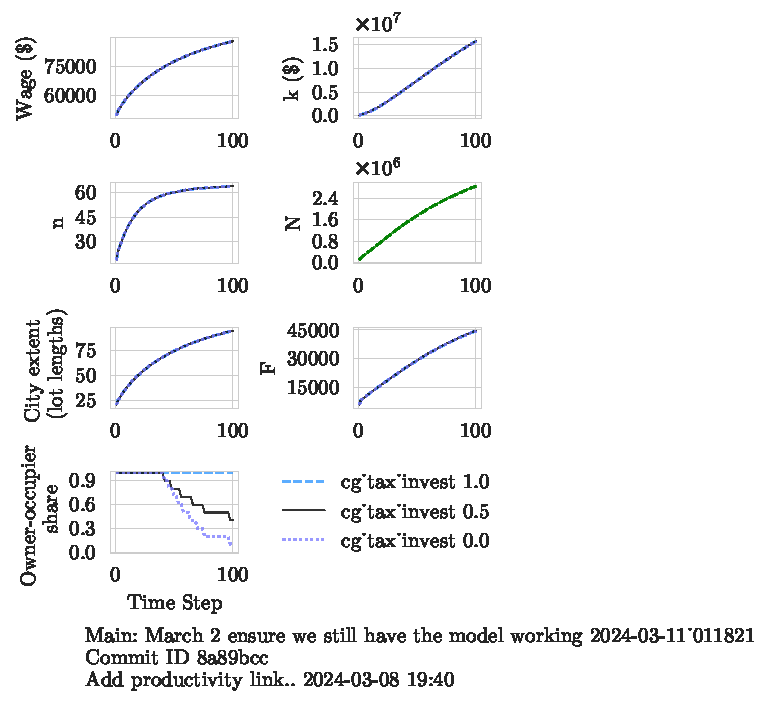
\includegraphics[scale=.6, trim={0 1.4cm 4.5cm 0},clip]{fig/cg_tax_invest-Main-011821.pdf} %\pause
    % 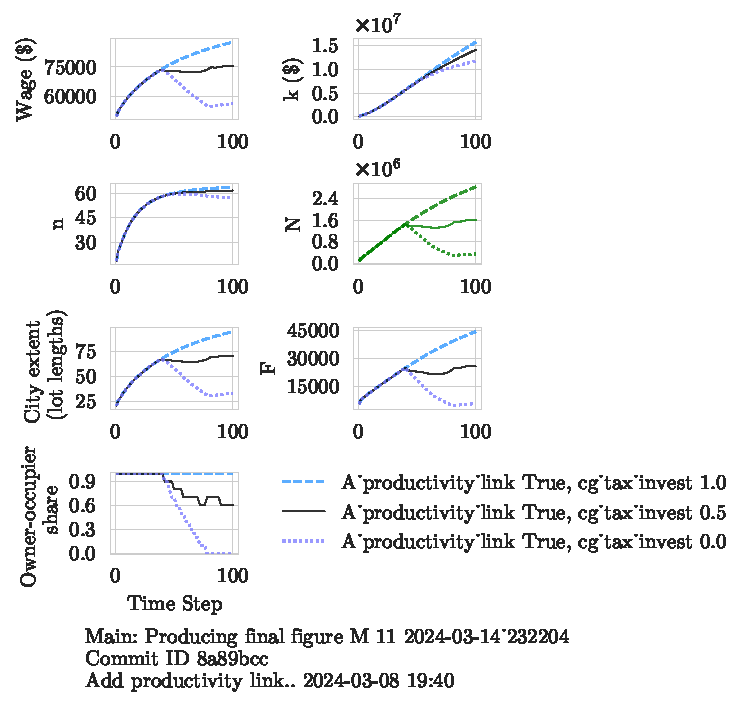
\includegraphics[scale=.6, trim={0 1.4cm 3.8cm 0},clip]{fig/With-productivity_linkcg_tax_invest-232204.pdf} 
    % \draw[color=white, fill=white] (8.3,-2.3) rectangle (12.6,-4.5);
\end{frame}% %

\note[enumerate]{\item Let's compare the result if there is feedback to productivity
\item Now the real variables are affected
\item With a 100\% tax the real economy follows the no spillover path a 100\% tax \textbf{insulates the economy} against the feedback.
\item We see rising tenantization reducing productivity, which pulls down the wage, which reduces city size.
\item With no capital gains tax on housing speculation, the economy crashes
\item complete financialization of the housing stock happens faster. 
\item With a 50\% rate financialization of the housing stock is slower. This is interesting. The slower growth reduces capital gains and makes speculation  less  profitable 
}

%%%%%%%%%%%%%%%%%%%%%%%%%%%%%%%%%%%%%%%%%%
\begin{frame}{The model tells us that}  \Large
\begin {itemize}[<+-|alert@+>]
 %\item In the absence of linkages between the housing market and the production sector, of the policy tools we consider, only density and transportation cost and capital gains taxation have much effect. 
 % \only<1>{\color{red}}
\item In the presence of linkages, policy tools can have dramatically different effects %. This is a potentially very important result. 
 % \pause

 % \only<2>{\color{red}}
\item  A capital gains tax on speculative investment without linkage increases owner occupancy 

 % \only<2>{\color{red}}
\item With a productivity linkage, a capital gains tax on speculation also increases wages and the size of the city
 % \pause
  % \only<3>{\color{red}}
\end{itemize}
\end{frame}

%%%%%%%%%%%%%%%%%%%%%%%%%%%%%%%%%%%%%%%%%
\begin{frame}{A capital gains tax on owner-occupiers}
 \centering 
\resizebox{12.0cm}{!}{%
    \begin{tikzpicture}
\node[inner sep=.5pt] (plain) at (0,0)
    {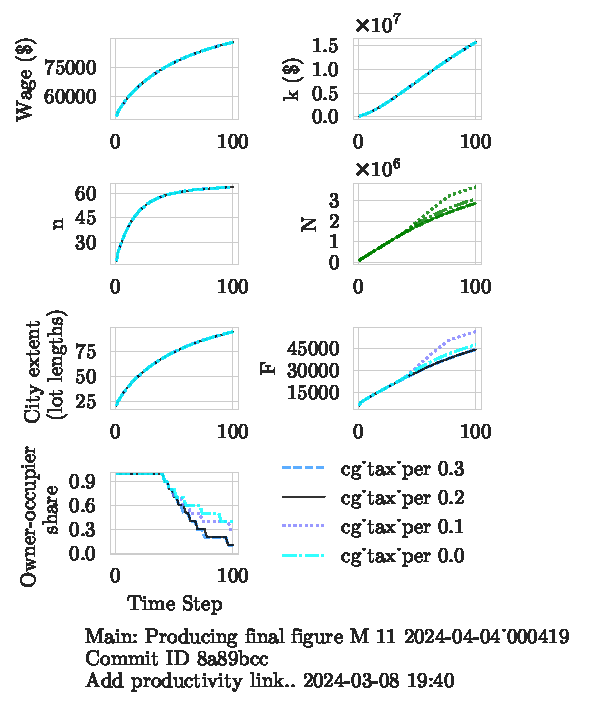
\includegraphics[height=10cm,%width=.5\textwidth,
    trim={.3cm 1.4cm 1cm 0},clip]{fig/cg_tax_per-000419.pdf}}; 

\node[inner sep=0pt] (link) at (7.6,0)
    {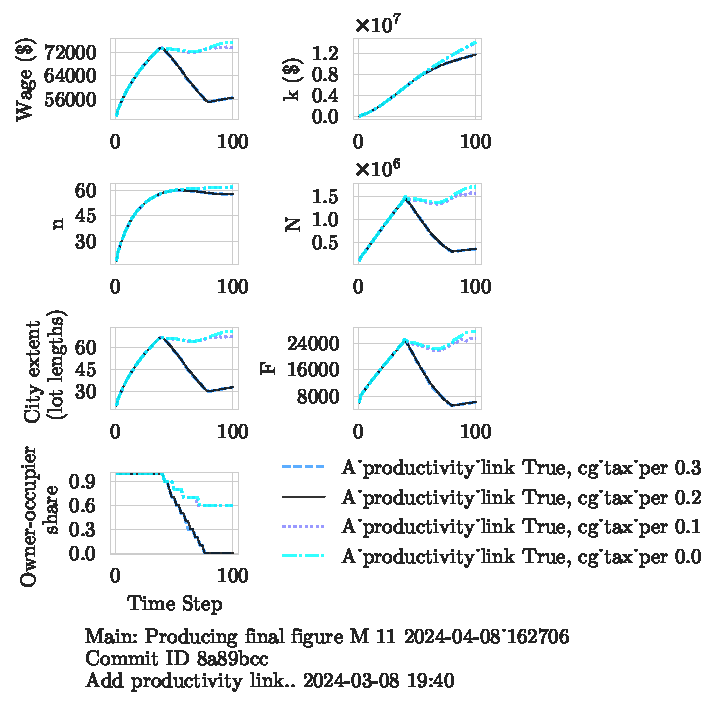
\includegraphics[height=10cm,%width=.5\textwidth, 
    trim={.1cm 1.4cm 4.cm 0},clip]{fig/link-cg_tax_per-4_162706.pdf}};
    
\draw[color=white, fill=white] (8.,-2.3) rectangle (12.6,-4.5);
\end{tikzpicture}
}
    %  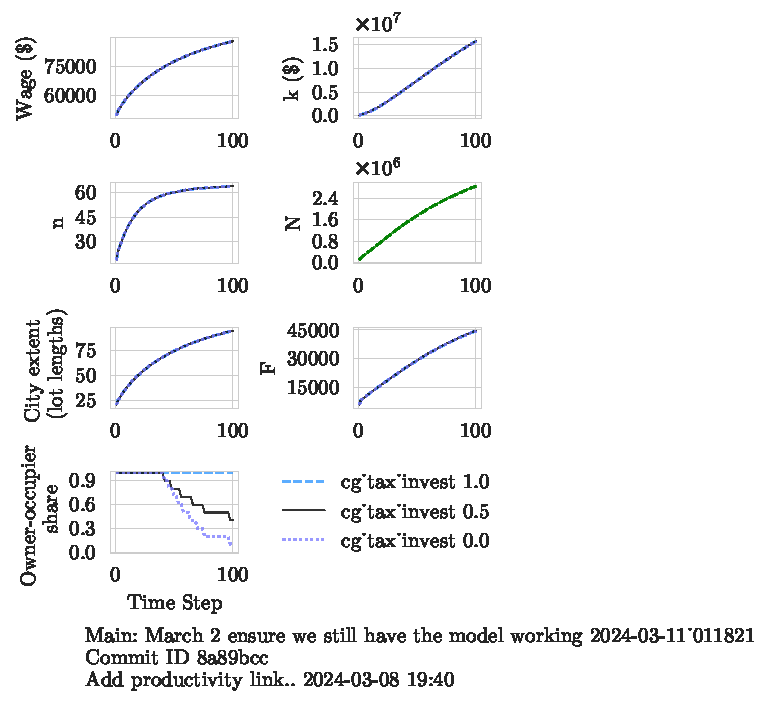
\includegraphics[scale=.55, trim={0 1.4cm 4.5cm 0},clip]{fig/cg_tax_invest-Main-011821.pdf} %\pause
    % 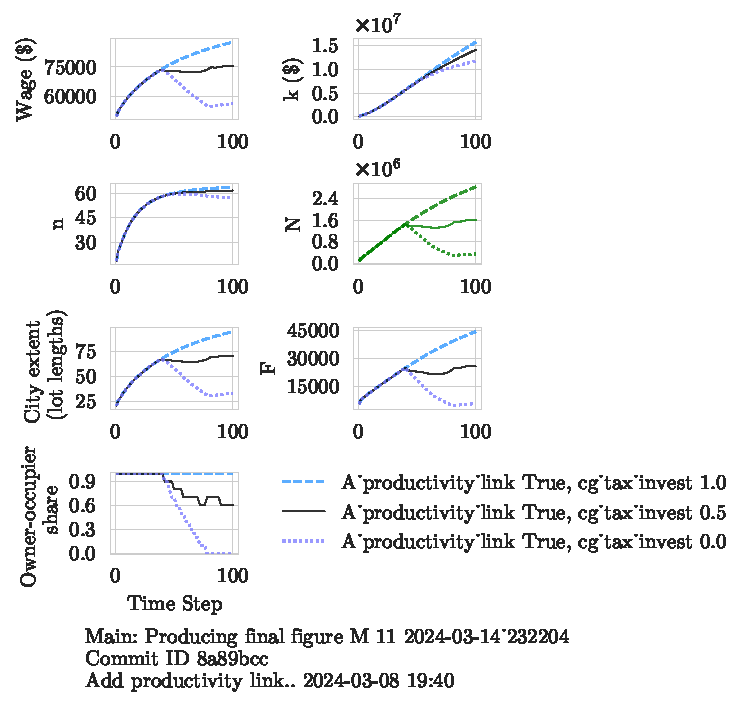
\includegraphics[scale=.55, trim={0 1.4cm 3.8cm 0},clip]{fig/With-productivity_linkcg_tax_invest-232204.pdf} 
\end{frame}% %

%%%%%%%%%%%%%%%%%%%%%%%%%%%%%%%%%%%%%%%%%
\begin{frame}{The model tells us that}  \Large
\begin {itemize}[<+-|alert@+>]
 %\item In the absence of linkages between the housing market and the production sector, of the policy tools we consider, only density and transportation cost and capital gains taxation have much effect. 
 % \only<1>{\color{red}}
\item  A capital gains tax on owner-occupiers above the level on investors has a powerfully negative effect on population and wages
\end{itemize}
\end{frame}

%%%%%%%%%%%%%%%%%%%%%%%%%%%%%%%%%%%%%%%%%
\begin{frame}{Summarizing other experiments} \Large
\begin {itemize}[<+-|alert@+>]
% \begin {itemize}[<alert@+>]\Large 

\item  The cost of capital has surprisingly little effect on any variables in either case

\item  Transportation cost has a strong effect on wages and city size as expected 
 
\item Low transportation costs with financial system spillovers appear to induce something like cyclical behaviour

\item  Increasing density increases the population but does not affect wages or city extent
\end{itemize}
\end{frame}% 


%%%%%%%%%%%%%%%%%%%%%%%%%%%%%%%%%%%%%%%%%%
\begin{frame}{Changing the cost of capital for investors}
 \centering 
\resizebox{12.0cm}{!}{%
\begin{tikzpicture}
\node[inner sep=.5pt] (plain) at (0,0)
    {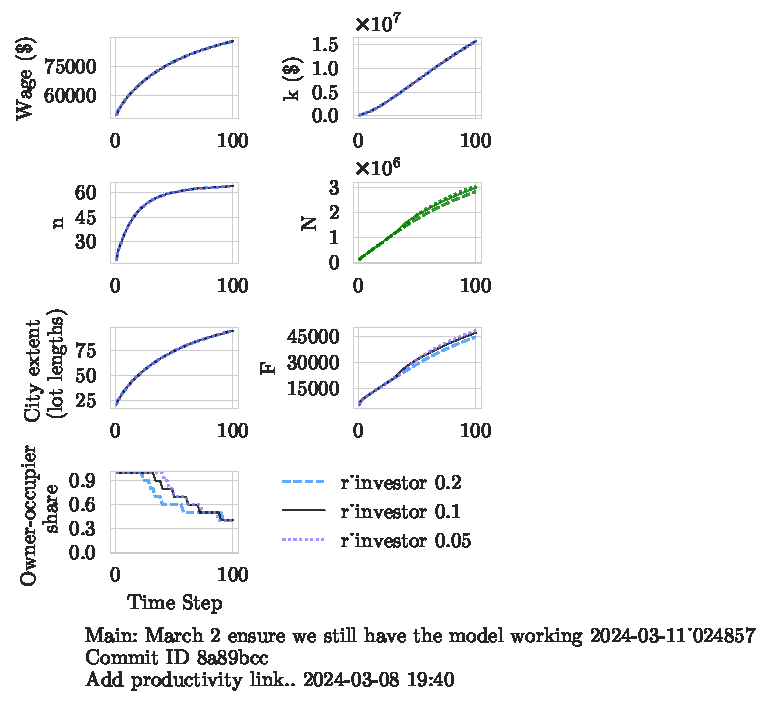
\includegraphics[height=10cm,%width=.5\textwidth,
    trim={.3cm 1.4cm 1cm 0},clip]{fig/r_investor-Main-024857.pdf}}; 


\node[inner sep=0pt] (link) at (6.,0)
    {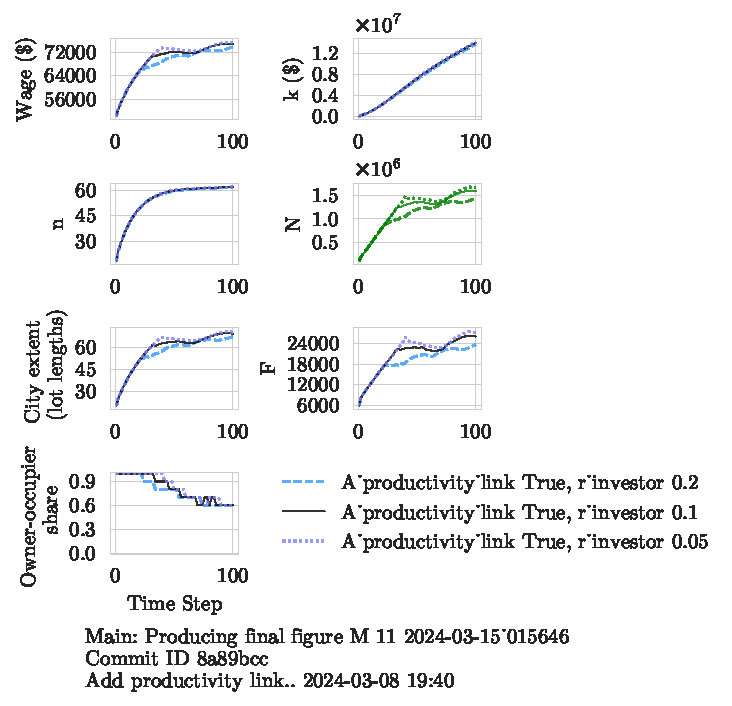
\includegraphics[height=10cm,%width=.5\textwidth, 
    trim={.1cm 1.4cm 4.cm 0},clip]{fig/With-productivity_link-r_investor-15_015646.pdf}};
    
\draw[color=white, fill=white] (6.2,-2.3) rectangle (10.6,-4.5);

\draw[red!50,line width=1mm] (-3.3,3.9) circle (1.75cm);
\draw[latex-,line width=1mm  ] (-2.1,4.5)--+(.5,.5)node[above right]{\Huge\$88,000};


\draw[red!50,line width=1mm] (4.8,3.9) circle (1.75cm);
\draw[latex-,line width=1mm  ] (6.1,4.5)--+(.5,.5)node[above right]{\Huge\$74,000};

%\draw[fill=yellow, line width=.25mm] (0,0) rectangle (-1.,2.5);
%\draw[red!90, line width=1mm] (8.4,1.35) circle (1.75cm);
%\draw (-.5,2.5)--()node[]{\$90,000};
\end{tikzpicture}
}

\end{frame}% %

\note[enumerate]
{
\item this seems to have little effect. I was surprised
\item We get the same dramatic effect with a productivity feedback: lower wage $\rightarrow$  half the population
}

%%%%%%%%%%%%%%%%%%%%%%%%%%%%%%%%%%%%%%%%%
\begin{frame}{Transportation costs}
 \centering 
\resizebox{11.0cm}{!}{%
\begin{tikzpicture}
\node[inner sep=.5pt] (plain) at (-2,0)
{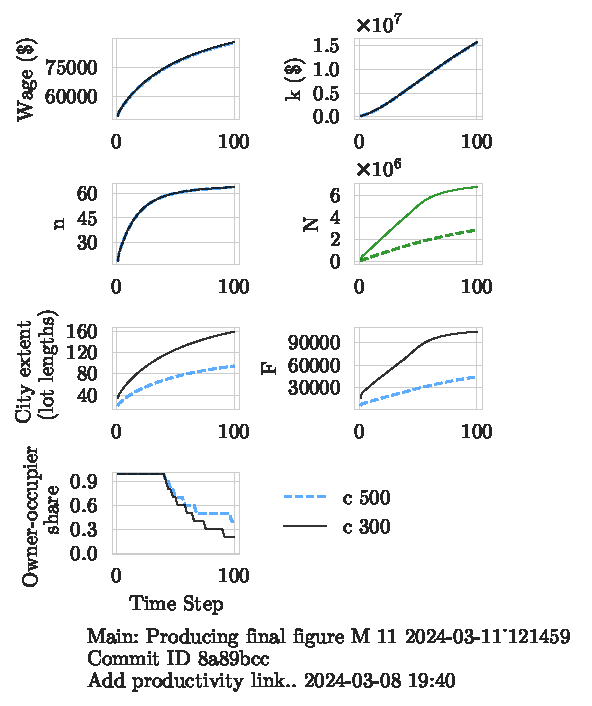
\includegraphics[height=11cm,%width=.5\textwidth,
trim={.2cm 1.4cm 1cm 0},clip]{fig/c-Main-121459.pdf}}; 

\node[inner sep=0pt] (link) at (6,0)
{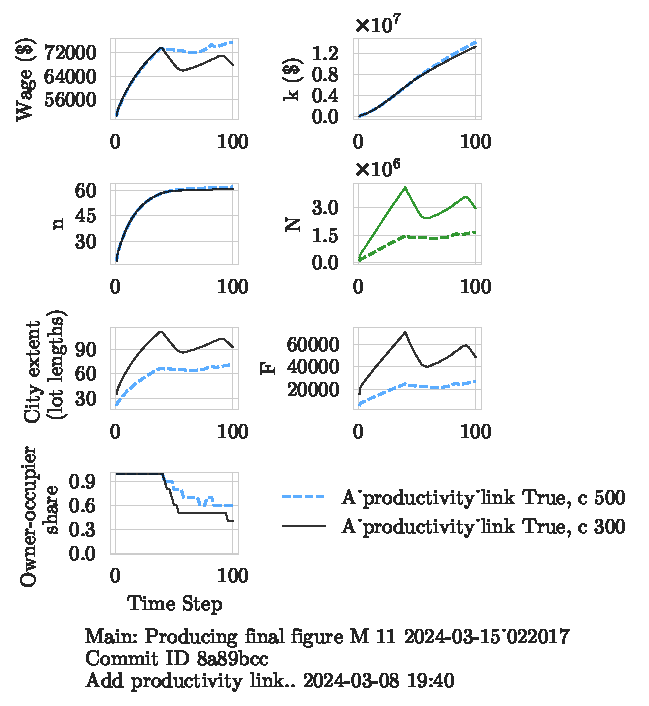
\includegraphics[height=10cm,%width=.5\textwidth, 
trim={0cm 1.4cm 2.5cm 0},clip]{fig/With-productivity_link-c-15_022017.pdf}};

\draw[color=white, fill=white] (6,-2.3) rectangle (10.2,-4.5);

\draw[red!50, line width=1mm] (0.2,1.35) circle (1.75cm);
\draw[red!90, line width=1mm] (8.4,1.35) circle (1.75cm);

\draw[latex-,line width=1mm  ] (8.,1.9)--+(-3,3.2)node[above ]{\Huge Cycles};
\end{tikzpicture}
}
\end{frame}% 
\note[enumerate]
{
\item The effects on city size is what we expect
\item in the lower left there is a higher ownership ratio with higher costs. The city is smaller and grows more slowly, so there is lower price growth and less speculative investment. 
\item The surprise here is that with feedback, lower transportation costs induce oscillations.
% \item What seems to be happening is that low transportation costs make the size of the city very sensitive to wage changes. A small rise adds many people and a sharp increase in investor ownership. This reduces productivity and drives down the wage and leads to a drop in speculation. 
}
%%%%%%%%%%%%%%%%%%%%%%%%%%%%%%%%%%%%%%%%%
\begin{frame}{Relaxing density restrictions}
 \centering 
\resizebox{11.5cm}{!}{%
   \begin{tikzpicture}
\node[inner sep=.5pt] (plain) at (-2,0)
    {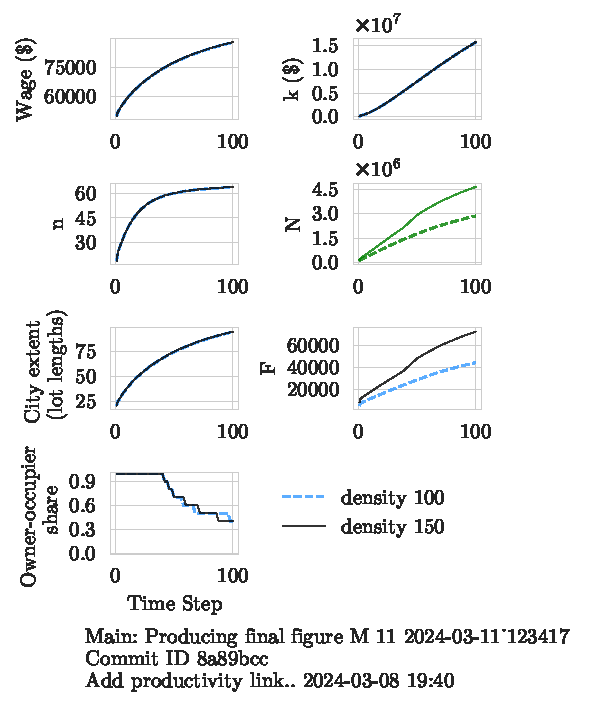
\includegraphics[height=10cm,%width=.5\textwidth,
    trim={.2cm 1.4cm 1cm 0},clip]{fig/density-Main-123417.pdf}}; 

\node[inner sep=0pt] (link) at (5.5,0)
    {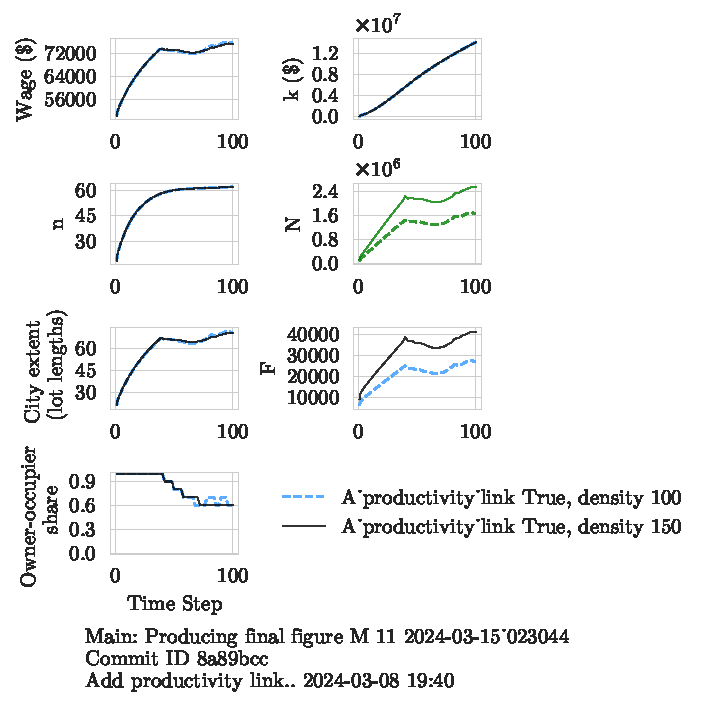
\includegraphics[height=10cm,%width=.5\textwidth, 
    trim={0cm 1.4cm 3.5cm 0},clip]{fig/With-productivity_link-density-023044.pdf}};
    
\draw[color=white, fill=white] (6,-2.3) rectangle (10.2,-4.5);

\draw[red!50,line width=1mm] (-3.6,-1) circle (1.65cm);
%\draw[latex-,line width=1mm  ] (-2.1,4.5)--+(.5,.5)node[above right]{\Huge\$88,000};

\end{tikzpicture}
}
\end{frame}% 

\note[enumerate]
{
\item Illustrates the effect of a population density of 100 and 150 per grid space.

\item The dashed line is low the solid line is higher density 

\item Without a productivity linkage the change increase population but not wages or city extent.  

\item with a productivity linkage wages are lower the city is smaller and we see signs of a financial boom-bust cycle.
}


%%%%%%%%%%%%%%%%%%%%%%%%%%%%%%%%%%%%%%%%%
\begin{frame}{The wealth sensitivity parameter}
 \centering 
\resizebox{12.0cm}{!}{%
\begin{tikzpicture}
\node[inner sep=0pt] (plain) at (0,0){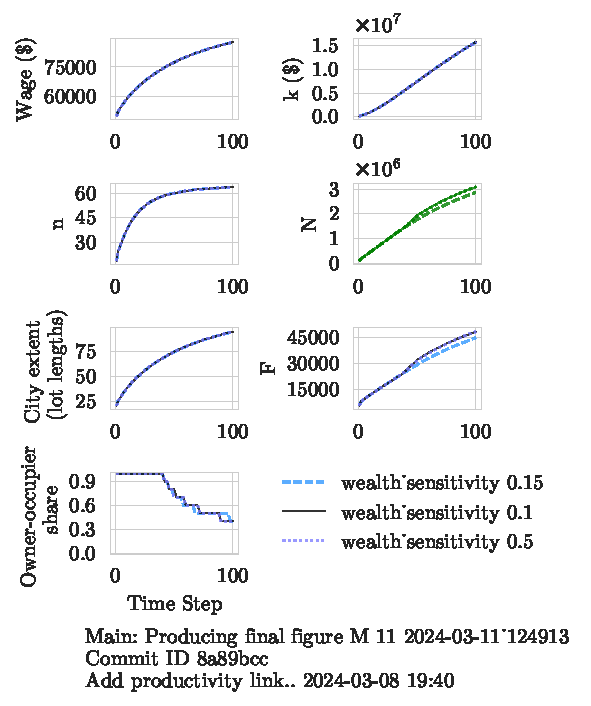
\includegraphics[width=.52\textwidth, trim={.3cm 1.4cm .8cm 0},clip]{fig/wealth_sensitivity-124913.pdf}}; 

\node[inner sep=0pt] (link) at (5.3,0)
{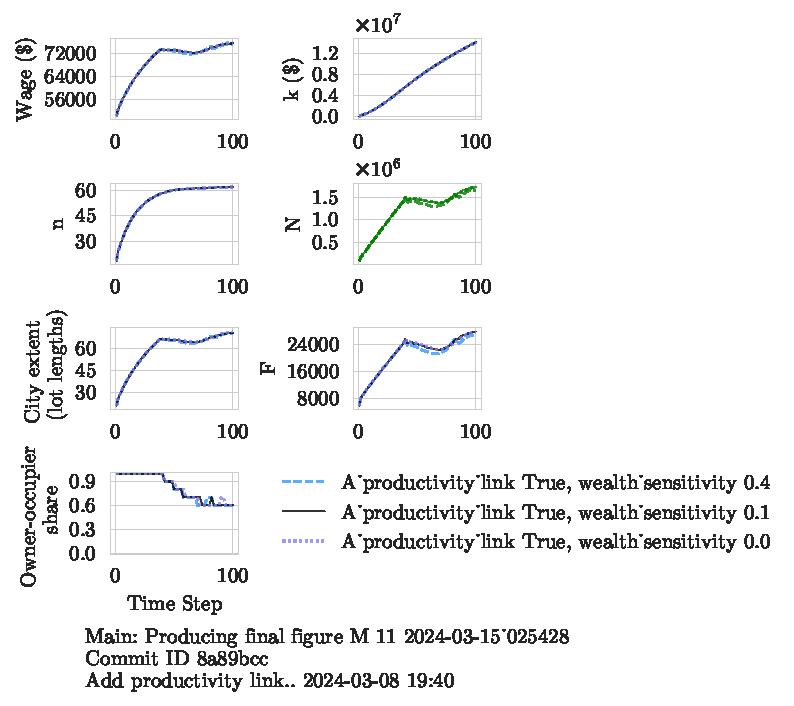
\includegraphics[width=.5\textwidth, trim={.1cm 1.4cm 4.75cm 0},clip]{fig/With-productivity_link-wealth_sensitivity-025428.pdf}};
\draw[color=white, fill=white] (5.5,-1.5) rectangle (8.6,-4);


\end{tikzpicture}
}
\end{frame}% 

\note[enumerate]
{
\item The wealth sensitivity parameter controls the wealth required for accessing a mortgage, and its effect is illustrated in Figure~\ref{fig:Wealth-based} in the model chapter.
\item The effect of the wealth sensitivity parameter seems to be pretty minimal.
\item with and without a productivity linkage, with wealth sensitivity parameter values of 0.1, 0.15, and 0.5. 
}

%%%%%%%%%%%%%%%%%%%%%%%%%%%%%%%%%%%%%%%%%
\begin{frame}{The property tax rate}
 \centering 
\resizebox{11.5cm}{!}{%
    \begin{tikzpicture}
\node[inner sep=.5pt] (plain) at (-2,0)
    {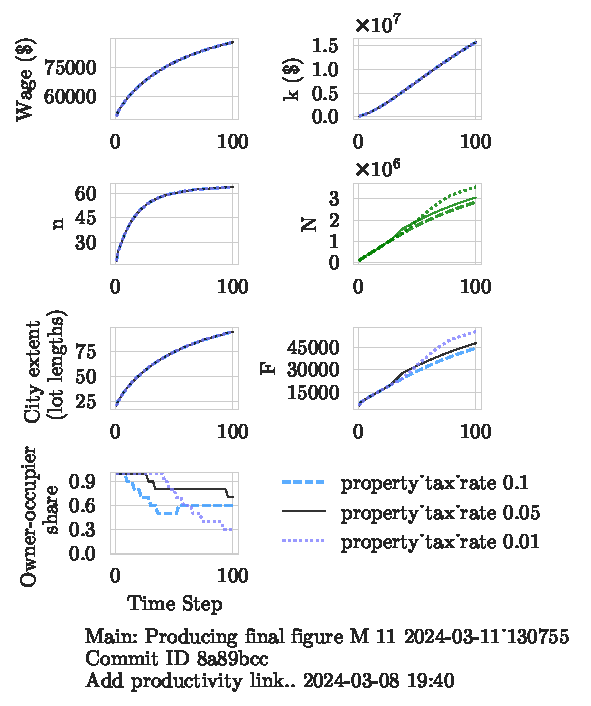
\includegraphics[height=10cm,%width=.5\textwidth,
    trim={.2cm 1.4cm .1cm 0},clip]{fig/property_tax_rate-Main-130755.pdf}}; 

\node[inner sep=0pt] (link) at (6,0)
    {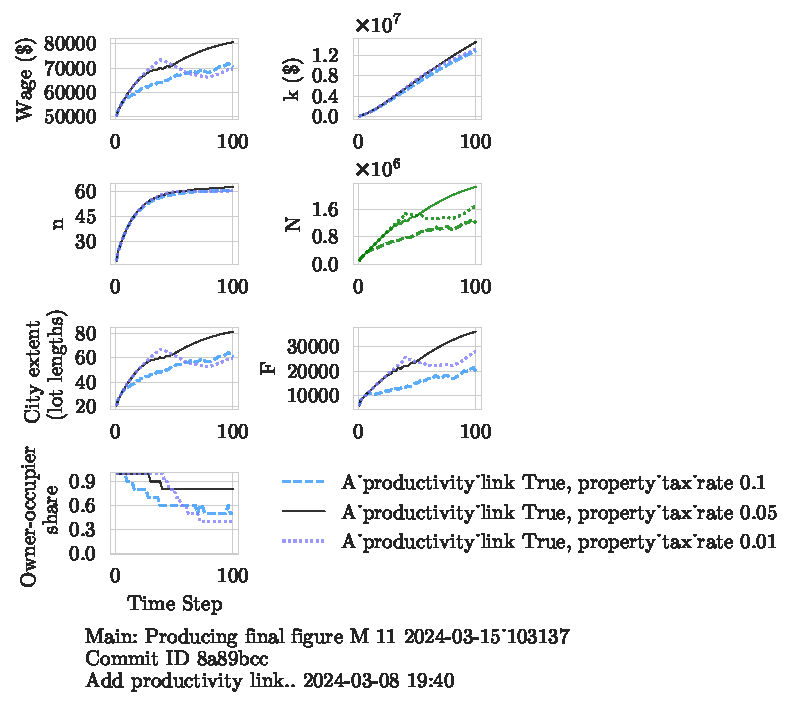
\includegraphics[height=10cm,%width=.5\textwidth, 
    trim={0cm 1.4cm 5.cm 0},clip]{fig/With-productivity_link-property_tax-103137.pdf}};
    
\draw[color=white, fill=white] (6,-2.3) rectangle (10.2,-4.5);


\draw[red!50,line width=1mm] (-4.1,-3.4) circle (1.65cm);
\draw[latex-,line width=1mm  ] (-3,-3.6)--+(1,-.8)node[ right]{\Large Crossover};
\end{tikzpicture}
}
\end{frame}% 
 \note[enumerate]{\item Comparing the effect of property tax rates between 1\% and 100\%. without a productivity linkage. 

 \item This is a specialized area that someone as naive as I am should not try to say much about.  

\item Both high and low rates appear to favour investors compared to what I think is a roughly realistic value. 

\item \textbf{CROSSOVER: I think very low rates subsidize investors and very high rates push out some owner-occupiers.} 
}

%%%%%%%%%%%%%%%%%%%%%%%%%%%%%%%%%%%%%%%%%
\begin{frame}{A 25-year reduction in the investor capital gains  tax}
 \centering 
\resizebox{9.0cm}{!}{%
    \begin{tikzpicture}

\node[inner sep=.5pt] (plain) at (0,0)
    {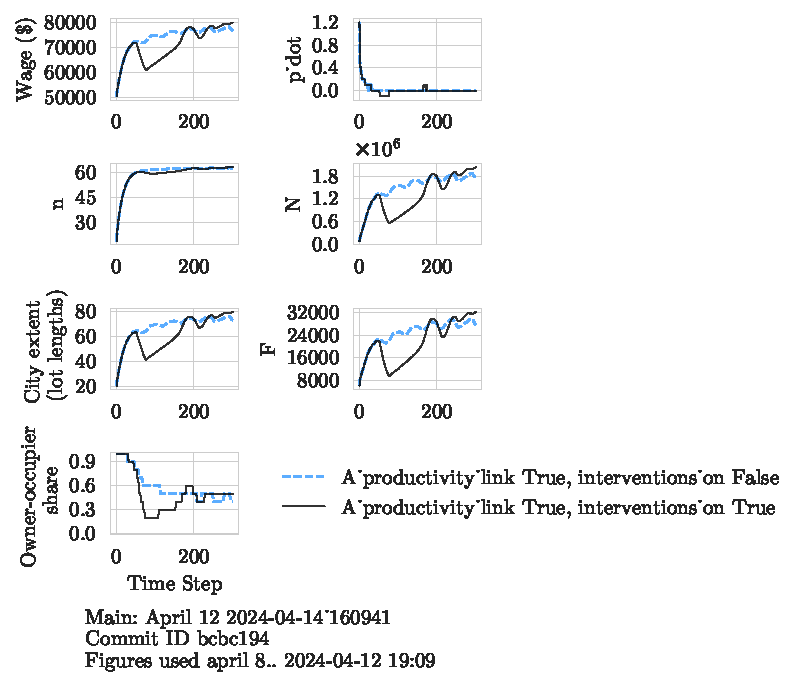
\includegraphics[height=8cm,%width=.5\textwidth,
    trim={.2cm 1.4cm 5.5cm 0},clip]{fig/Link-CGI-15-0-100-300-years.pdf}}; 

% \node[inner sep=0pt] (link) at (6,0)
%     {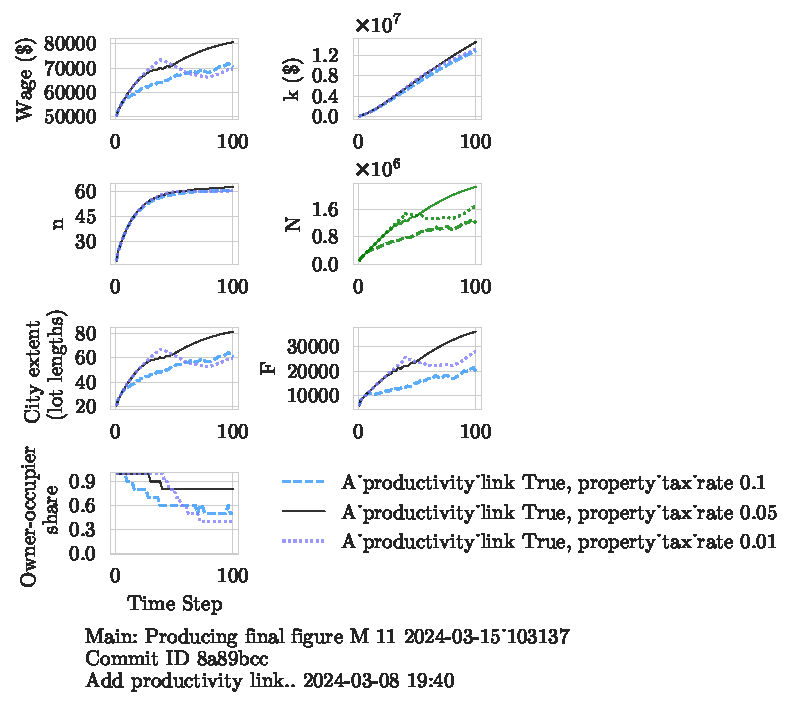
\includegraphics[height=10cm,%width=.5\textwidth, 
%     trim={0cm 1.4cm 5.cm 0},clip]{fig/With-productivity_link-property_tax-103137.pdf}};

%\draw[step=.5, thin, gray!30] (-5,-5) grid (5,5);

\begin{scope}[shift={(1.,-3.35)}]
\draw[color=white, fill=white, fill= white] (0,0) rectangle (2.8,1.5);   %, fill=white]
\node at (1.6,1.05)[align=left, scale=01.2]{\tiny 15\% capital gains tax};
\node at (2.2,.58)[align=left,  scale=01.2]{\tiny temporary zero then 100\% tax};
\end{scope}

\end{tikzpicture}
}
 %     \caption[The effect of temporarily reducing the capital gains tax for investors from 15\% to zero for 25 years]{The effect of temporarily reducing the capital gains tax for investors from 100\% to zero for 25 years, with the productivity linkage. The black line shows the case with the policy shock. The blue dashed line shows the reference case in which the original 15\% capital gains tax is maintained.}
\end{frame}% 
\note[enumerate]
{
\item This is a bit different - A 300 year run and a 25-year shock=at year 50
\item With a productivity linkage
\item the blue line is the no-shock case. It shows regular speculative cycling
\item The black line shows the effect f a policy shock.
\item we start with a 15\% capital gains tax for investors. A (conservative?) government drops it to zero, and then (a populist government?) raises it to 100\% 
\item the result is a major setback for the city followed by a very slow recovery. 


}
% %%%%%%%%%%%%%%%%%%%%%%%%%%%%%%%%%%%%%%%%%
% \begin{frame}{Result}

% \end{frame}% 
% %%%%%%%%%%%%%%%%%%%%%%%%%%%%%%%%%%%%%%%%%%

\begin{frame}{Results} \Large
\begin {itemize}[<+-|alert@+>]
\item A restrictive mortgage market does not affect the production sector or city size

\item  Increasing property taxes reduces owner-occupiers, but has only a small effect on city size when there is no linkage 
 
\item  With linkage increasing property taxes depresses wages, population, and city size
\end{itemize}
\end{frame}% %----------------------------%

% %%%%%%%%%%%%%%%%%%%%%%%%%%%%%%%%%%%%%%%%%
% \begin{frame}{}
%   \centering \Large
%   \emph{Future Work}
% \end{frame}
% %%%%%%%%%%%%%%%%%%%%%%%%%%%%%%%%%%%%%%%%%
% \begin{frame}{Extensions}
%  \begin{center}
%     \begin{minipage}{0.6\textwidth}
%  \hspace{3cm}\begin{itemize}\Large 
%       \item a competing city
%       \item housing production sector
%       \item household types
%       \item housing types
%       \item multiple industries
%       \item zoning effects
%       \item \dots
%   \end{itemize}
%  \end{minipage}
%   \end{center}
% \end{frame}
%%%%%%%%%%%%%%%%%%%%%%%%%%%%%%%%%%%%%%%%%
\begin{frame}{Final comments}
 \begin{itemize} \Large
\item There is a gap in economic theory around who gets urban rents and why that matters
\item I partly bridge this gap by combining from several  fields:

    \begin{enumerate}\item Jacobs agglomeration
    
    \item The scale literature 
    
    \item Neoclassical growth theory
    
    \item Neoclassical production theories
    
    \item Alonso-style urban analysis
    
    \item Ricardian rent theory
    \end{enumerate}
\end{itemize}
\end{frame}
%%%%%%%%%%%%%%%%%%%%%%%%%%%%%%%%%%%%%%%%%
\begin{frame}{} 

\begin{itemize} \Large
\item The model is modular and extensible
\item It allows us to explore a variety of policy interventions 
\item It tells us that: 
\begin{enumerate}
    \item Financial interests are likely to take over much of the land and capture much of the surplus generated by the city
    \item The capture of urban value by financial actors affects the social class and may affect urban productivity
    \item Public policies will have different effects if financialization affects productivity
    \end{enumerate}
\end{itemize}
\end{frame}
%%%%%%%%%%%%%%%%%%%%%%%%%%%%%%%%%%%%%%%%%
\begin{frame}
  \centering \Large
  \emph{Thank You!}
\end{frame}
%%%%%%%%%%%%%%%%%%%%%%%%%%%%%%%%%%%%%%%%%

\end{document}
%%%%%%%%%%%%%%%%%%%%%%%%%%%%%%%%%%%%%%%%%
%%%%%%%%%%%%%%%%%%%%%%%%%%%%%%%%%%%%%%%%%

